\graphicspath{{../../pictures/medecine/}}

\usetikzlibrary{quotes}

\section{Définitions}%
\label{sec:definitions}

\begin{figure}
  \centering
  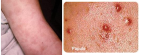
\includegraphics[width=0.8\linewidth]{160_macule_papule}
  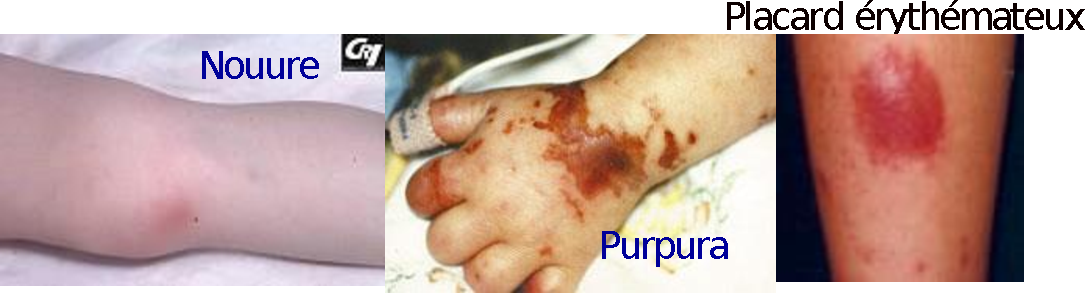
\includegraphics[width=0.8\linewidth]{160_purpura_placard}
  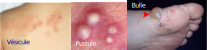
\includegraphics[width=0.8\linewidth]{160_vesicule}
\end{figure}

Morbiliforme = avec intervalles de peau saine\\
Scarlatiniforme = sans intervalles de peau saine


\section{4 - Sécurité du patient}%
\label{sec:ue_1_item_4_securite_du_patient}

Infection nosocomiale : > 48h post-admission ( > 30 j après opération, > 1 an si
pose de matériel étranger)

Agents infectieux : \bact{ecoli}, \bact{dore}, \bact{aeruginosa}

\begin{table}[htpb]
  \centering
  \caption{Précautions}
  \begin{tabular}{ccc}
    \toprule
    Air & Gouttelettes & Contact  \\
    \midrule
    masque FFP2 & masque chir & tablier \\
    tuberculose, rougeole & grippe, ménigocoque & BMR, SARM, varicelle...\\
    varicelle & coqueluche, mycoplasme, rubéole, & \\
    & oreillons, parvorvirus B19, VRS & \\
    \bottomrule
  \end{tabular}
\end{table}

ATB :
\begin{itemize}
  \item prophylaxie pour Altemeier 1-2 (\{pas de, faible\} rupture d'asepsie
    resp.)
  \item curatif pour Altemeier 3-4 (\{trauma < 4h contamination digestive,
    trauma > 4h, contamination fécale\}, 
\end{itemize}

Cathéter : changer 72h
\section{UE2 - 26 : Prévention des risques foetaux}%
\label{sec:ue2_item_26_prevention_des_risques_foetaux}

\begin{table}[htpb]
  \centering
  \caption[dummy]{Dépistage obligatoire.\\
  \dag: pas de sérologie (hémoc + PL chez NN)}
  \begin{tabular}{*{4}{c}}
    \toprule
    Infection & Dépistage & Prévention primaire & Prev. secondaire \\
    \midrule
    Toxoplasmose & 10 SA & Hygiène & Spiramycine ou Pyriméthamine\\
    & mensuel si non immun & & \\
    \midrule
    Rubéole  & < 10 SA, 20 SA & ROR & \\
    & & Pas de vaccin pendant grossesse & \\
    \midrule
    VHB & 6M & lamivudine/ténofovir & vaccin \\
    strept.\dag B & 34-38 SA & amoxicilline & \\
    syphilis & 1er trimestre & &pénicilline G retard\\
    \bottomrule
  \end{tabular}
\end{table}

\begin{table}[htpb]
  \centering
  \caption[dummy]{Dépistage non obligatoire.\\
  \dag: pas de sérologie (hémoc)}
  \begin{tabular}{*{3}{c}}
    \toprule
    Infection & Prévention primaire & Prev. secondaire \\
    \midrule
    VIH  & & antirétroviral, AZT (foetus)\\
    CMV (frequent) & hygiène & \\
    HSV & & (val)aciclovir (césarienne ?)\\
    Rougeole & ROR & Ig (sous 6 j) \\
    Varicelle & vaccin & Ig (sous 96h) \\
    Listériose & hygiène & amoxicilline \\
    \bottomrule
  \end{tabular}
\end{table}

\paragraph{Autres} : paludisme [urgence \skull (quinine-artésunate IV)], IU, \bact{burnetii}
[pas de lait cru], parvovirus B19 [surveillance], vaginose [métronidazole],
arbovirus
\section{143 - Vaccination}%
\label{sec:item_143_vaccination}

Vaccins acellulaire : coqueluche\\
Vaccins anatoxine : diphtérie-tétanos\\
Vaccins entier: polio,grippe, VHA, rage
\subsection{Enfant}%
\label{sub:enfant}

\begin{table}[htpb]
  \centering
  \caption{Vaccins obligatoires pour l'enfant}
  \begin{tabular}{*{7}{c}}
    DTP + Coqueluche & 2M & 4M & 11M & & 6A & 11-13A\\
    \bact{influenzae} & 2M &4M & 11M \\
    VHB & 2M & 4M & 11M \\
    Pneumocoque & 2M & 4M & 11M \\
    Méningocoque C & & 5M & 12M\\
    ROR & & & 12M & 16-18M\\
  \end{tabular}
\end{table}

Rattrapages :
\begin{itemize}
  \item VHB : 3 doses (16M - 11A), 2 doses (11-15A)
  \item Méningocoque C : 1 dose (16M - 24A)
  \item HPV : 3 dose (15-19A)
  \item ROR : nb doses manquantes (11A)
\end{itemize}

\subsection{Adulte}%
\label{sub:adulte}

\begin{table}[htpb]
  \centering
  \caption{Vaccins recommandés pour l'adulte}
  \begin{tabular}{*{5}{c}}
    DTP & 25A & 45A & 65A & 75, 85...A\\
    Coqueluche & 25A \\
    Grippe& & & & 65,66...A\\
    Zona& & & & 1 dose (65-74A)\\
  \end{tabular}
\end{table}

Post-exposition : tétanos [vaccin +/- Ig], VHA, méningocoque (A,B,C,Y ou W135), rage [vaccin +/-
Ig], rougeole (72h, sauf femme enceinte = Ig)

Contre indications :
\begin{itemize}
  \item permanente : allergie oeuf (fièvre jaune, grippe), immunodéprimé
    \item temporaire : infection aigüe grave, pas de vaccin vivant pour la femme
      enceinte, 3 mois après Ig
\end{itemize}

Réactions :
\begin{itemize}
  \item bénigne : vivant = infection retardée, inerte = inflammation locale
    immédiate
    \item grave : anaphylactique, maladie infectieuse, dysimmunitaires
\end{itemize}

\subsection{Grossesse}%
\label{sub:grossesse}

Recommandé : grippe

Possible : inactivé (tétanos, diphtérie, VHA, VHB, méningo, pnemoc...), vivant
atténué (fièvre jaune si voyage obligatoire)

Contre-indiqué : Varicelle, ROR (2 mois avant grossesse mais possible en début)
\section{144 - Fièvre aigüe}

Fièvre : \(\ge 38^{o}\) matin, \(38.3^{o}\) soir [+0.5$^{o}$ si axillaire/buccal]
\begin{itemize}
\item aigüe si \textless{} 5 jours
\item prolongée si \textgreater{} 20 jours
\end{itemize}

\danger fièvre \(\neq\) infection

\begin{figure}[htpb]
  \centering
  \resizebox{\linewidth}{!}{
    \tikz \graph [
  % Labels at the middle 
      edge quotes mid,
  % Needed for multi-lines
      nodes={align=center},
      sibling distance=3cm,
      edges={nodes={fill=white}}, 
    layered layout]
    {
      Point d'appel évident -> {
        oui -> {
          Virose banale -> Ttt symptomatique [draw] -> "Réévalution 48-72h";
          Foyer bactérien -> Ttt étiologique [draw] -> "Réévalution 48-72h";
        };
        non  -> {
          "Sepsis grave\\Choc septique ?"[level distance=1.8cm] ->["oui"] 
          "ATB probabiliste\\Remplissage vasc.\\TDM, TAP urgence" [draw]; 
          "Sepsis grave\\Choc septique ?" ->["non"] 
          "Réévaluation\\Hospitalisation \\si terrain à risque";
          "Neutropénie\\asplénie" -> "Hémocultures\\ATB probabiliste" [draw];
          non infectieux -> {Hyperthermie, Autres};
        };
      };
    };
  }
  \caption{Démarche diagnostique}
\end{figure}

Signes de gravité :

\begin{itemize}
\item
  neuro: angoisse, agitation, confusion, troubles du comportement, coma
\item
  cardiovasc : FC > 120/min, TA systol < 90 mmHg,
  PAM < 65 mmHg
\item
  cutané : purpura, extrémités froides et cyanosées, marbrures
\item
  respiratoire : polypnée > 24/min, tirage, balancement
  thoraco-abdominal, polypnée superficielle, \(SaO_2 < 90 \%\)
\end{itemize}

Peut décompenser une comorbidité :

\begin{itemize}
\tightlist
\item
  neurologique
\item
  \(37 + n^\circ\) =\textgreater{} \(+400\cdot n\) mL/j pertes hydriques
\item
  \(37 + n^\circ\) =\textgreater{} \(+10 \cdot n\) battements/min pour
  FR et FC
\item
  augmentations des besoins en oxygène
\end{itemize}

Terrain à risque : femme enceinte, immunodépression

\danger ATB sans diagnostic seulement pour sepsis/grave, choc septique,
neutropénie (\(< 500 PNN/mm^3\)), asplénie, pupura fulminans

Traitement sympotmatique :~antipyrétiques seulement si fièvre mal
tolérée/terrain particulier =\textgreater{} paracétamol (aspirine, AINS
non recommandés)

\section{145 - Infections naso-sinusiennes}%
\label{sec:item_145_infections_naso_sinusiennes}

Rhinopharyngite virale =  99\%. Contagieux++ (goutelettes)

\paragraph{Clinique} rhume banal + fièvre, myalgie + inflammation muqueuses respiratoire

Peut rarement se compliquer en sinusite bactérienne (\bact{pneumocoque},
\bact{influenzae})
\begin{itemize}
  \item maxillaire++
  \item frontale, ethmoïdale, sphénoïdale (complication possible)
\end{itemize}
Y penser si 
\begin{itemize}
  \item fièvre $\ge 3$ jours
    \item 2 parmi 3 critères : douleurs $\ge 48$h, douleur unilatérale,
      augmentation rhinorrhée et purulence
\end{itemize}

\paragraph{Traitement}%
\label{par:traitement}
\begin{itemize}
  \item paracétamol, sérum phys. (pas d'AINS !)
  \item ATB seulement pour les sinusites bactériennes = amoxicilline ou
    amoxicilline-acide clavulanique si échec ou non maxillaire
\end{itemize}
\section{146 - Angines}%
\label{sec:item_146_angines}

Diagnostic clinique : fonctionnel (odynophagie, otalgie réflexe), physique
(fièvre, inflammation oropharynx + amygdale, adénopathies satellites sensibles)

Traitement ATB : seulement pour SGA\footnote{streptocoque $\beta$-hémolytique du groupe A}, l'angine de Vincent, diphtérie, gonocoque,
chancre syphilitique

\subsection{Érythémateuse/érythémato-pultacées}%
\label{sub:erythemateuse_erythemato_pultacees}
80-90\%

Étiologie = EBV, VIH (virus) ou SGA

Score de McIsaac : 1 point pour fièvre $> 38^{\circ}$, pas de toux, adénopathie
cervicale sensible, atteinte amygdale. -1 point si $\ge 45$ ans.

\begin{figure}[htpb]
  \centering
  \caption{Prise en charge}
  \tikz \graph[
  % Labels at the middle 
  edge quotes mid,
  % Needed for multi-lines
  nodes={align=center},
  sibling distance=3cm,
  edges={nodes={fill=white}}, 
  tree layout]
{
    "" -> {
      "McIsaac < 2" -> ttt symptomatique [level distance=2cm];
      "Enfant\\ou McIsaac $\ge$ 2" -> TDR [level distance=2cm]-> {
        "Dépistage VIH ?" -> ttt symptomatique [>"négatif"];
        "Amoxicilline\\(C2G/C3G)" [>"positif", draw];
      };
    };
  };
\end{figure}

\subsection{Pseudo-membraneuse}%
\label{sub:pseudo_membraneuse}

\paragraph{Mononucléose infectieuse} : fréquent, évolution bénigne

Examens : MNI-test et sérologie si négatif (IgM anti-VCA)

\paragraph{Diphtérie} : rare mais urgence \skull

Clinique : 
\begin{itemize}
  \item voyage en Europe en l'Est/développement, pas de vaccins, < 7 jours
  \item fausses membranes envahissant la luette
\end{itemize}

Examens : prélèvement puis ED + culture (corynébactéries) + PCR

Traitement : sérum puis vaccins + amoxicilline. Précautions gouttelettes

\subsection{Vésiculeuses}%
Toujours virales. Bénignes


\subsection{Ulcéreuses/ulcéro-nécrotiques}
Angine de Vincent (fréquent++) 
\begin{itemize}
  \item clinique puis confirmé par association fusospirillaire (ED).
  \item risque de complications locales
  \item amoxicilline
\end{itemize}

Chancre syphilitique : cf~\nameref{sub:syphilis}

Agranulocytose

\section{147 - Otites}%
\label{sec:otites}
\subsection{Otite moyenne aigüe}%
\label{sub:otite_moyenn_aigue}
Oedème de la trompe d'Eustache $\to$ otite congestive $\to$ otite purulente

\bact{pneumocoque}, \bact{influenzae}

Diagnostic : fièvre, signes généraux + otoscopie surtout (épanchement
rétro-tympanique si purulente, congestion si congestive)

Traitement : 
\begin{itemize}
  \item ATB seulement pour OMA purulente chez enfant $\le 2$ ans ou adulte si
symptomatologie bruyante
$\rightarrow$ amoxicilline per os (+acide clavulanique si otite et conjonctivite)
\item paracétamol (pas d'AINS, corticoïdes !)
\end{itemize}

Suivi 48-72h : échec si persistance des symptôme $\rightarrow$ amoxicilline +
acide clavulanique (si 1er traitement = amoxicilline). Au 2eme échec :
spécialiste

\subsection{Otite externe nécrosante}%
\label{sub:otite_externe_necrosante}

Bénigne : traitement local + antalgique\\
Nécrosante chez immunodéprimé + polype $\to$ avis ORL en urgence \skull

\subsection{Otite séromuqueuse}%
\label{sub:otite_seromuqueuse}
Inflammation chronique $\rightarrow$ épanchement non purulent. Fréquent chez
l'enfant. Adulte: chercher tumeur du cavum.

Diagnostic : hypoacousie, tympans mats

Guérison spontanée, pas d'ATB.

\subsection{Otites cholesteatomateuse}%
\label{sub:otites_choestatomateuse}
Non infectieux. 

Diagnostic : otorrhée fétide chronique, intermittente.

Traitement chirurgical, pas forcément réversible.


\section{148 - Méningites, méningo-encéphalites}

Signes de gravité :

\begin{itemize}
\item purpura extensif
\item trouble de la conscience (Glasgow \textless{}= 8)
\item signes de focalisation neuro
\item signes de souffrance du tronc cérébral
\item état de mal convuslif
\item instabilité hémodynamique
\end{itemize}

Contre-indication à la PL :

\begin{itemize}
\item
  anomalie de l'hémostase {[}PL dès stabilité{]}
\item
  instabilité hémodynamique {[}PL dès stabilité{]}
\item
  signe d'engagement cérébral (mydriase unilatérale, hoquet, trouble
  ventilatoire, enroulement) {}
\item
  crise convulsive récente
\item
  risque d'engagement cérébral (localisation neuro, trouble vigilance +
  Glasgow \textless{}= 11) {}
\end{itemize}

\subsection{Méningite}
Épidémio : virale dominent < 65 ans. Bactérienne dominent > 65 ans (70\% de
pneumocoque > 40 ans, 50\% sinon). Herpétique :
80\% < 20 ans ou > 50 ans

\begin{figure}[htpb]
  \centering
  \begin{subfigure}{0.4\textwidth}
    \resizebox{\textwidth}{!}{
      \tikz \graph [
  % Labels at the middle 
        edge quotes mid,
  % Needed for multi-lines
        nodes={align=center},
        sibling distance=3cm,
        edges={nodes={fill=white}}, 
      layered layout]
      {
        "Signes de localisation, crises comitiales, Glasgow $\le$ 11 ?" [level
        distance=2cm ]
   %->["oui"] "Hémocultures" [draw]->  "DXM+ATB" [draw] -> scanner [draw]-> PL[draw] ;
        ->["oui"] "Hémocultures\\DXM+ATB\\scanner" [draw]->["pas CI"] PL[draw] ;
        "Signes de localisation, crises comitiales, Glasgow $\le$ 11 ?" 
        ->["non"] "CI PL ?";
        "CI PL ?" [level distance=2cm] ->[left, "résolution"] PL [align here];
        PL-> {
          "bactérien ?" -> "ATB + DXM" [draw];
          "viral ?"  -> {
            "méningo-\\encéphalite"  -> aciclovir [draw];
            méningite -> symptomatique [draw];
          };
          "autres ?";
        };
      };
    }
    \caption{Traitement}
  \end{subfigure}
  \begin{subfigure}{0.58\textwidth}
    \resizebox{\textwidth}{!}{
      \tikz \graph [
  % Labels at the middle 
  %edge quotes mid,
  % Needed for multi-lines
        nodes={align=center},
  %edges={nodes={fill=white}}, 
      layered layout]
      {
        PL [draw] -> 
        "ED Gram\\culture + antibiogramme\\Coloration Ziehl-Neelsen $\rightarrow$
        PCR BK" [draw, align=left] 
        -> {
          "Suspicion méningite\\ bactérienne" [level distance=2cm ]
          ->["forte"] "Ag\\pneumocoque" [draw, level distance=2cm ] 
          -> ["négatif"] "PCR méningocoque" [draw];
          "Suspicion méningite\\ bactérienne" 
          ->["faible"] "PCR\\entérovirus LCS" [draw];
          "Autres" -> {"cryptocoque (ID), Lyme,\\VDRL-TPHA, leptospirose"};
        }
      };
    }
    \caption{Orientation}
  \end{subfigure}
\end{figure}

\begin{figure}[htpb]
  \centering
  \begin{minipage}{0.42\textwidth}
    \resizebox{\textwidth}{!}{

      \tikz \graph [
      layered layout]
      {
        LCS -> {
          purulent [level distance=1.5cm] -> {bactérien; "début viral"; };
          clair ->["normo",swap] viral ;
          clair ->["hypoglycorachie"] "Listeria, BK";
        }
      };
    }
  \end{minipage}
  \begin{minipage}{0.69\textwidth}
    \resizebox{\textwidth}{!}{

      \tikz \graph [
        nodes={align=center},
      layered layout]
      {
        ED LCS -> {
          positif ->
          {"diplocoque\\Gram+" -> pneumocoque -> "C3G + DXM" [draw];
            "diplocoque\\Gram{-}" -> méningocoque -> "C3G + DXM" [draw];
            "bacille\\Gram+" -> Listeria -> "amoxicilline\\+gentamicine" [draw];
          };
          negatif -> C3G + DXM [draw];
          negatif ->["Listeria ou signes de gravité"] "C3G + DXM\\(+ amoxicilline\\+
          gentamicine)"[draw];
        };
      };
    }
  \end{minipage}
\end{figure}

\begin{figure}[htpb]
  \centering
  
\includegraphics[width=0.8\linewidth]{../../pictures/medecine/148_antibio}
  \caption{Début des antibiotiques}
\end{figure}

\begin{table}[htpb]
  \centering
  \caption{Aspect LCS}
  
  \begin{tabular}{*{4}{c}}
    \toprule
    &normal & purulent & liquide clair \\
    \midrule
    Aspects & clair & trouble & clair \\
    Elements & < 5/\(mm^3\) & > 20/\(mm^3\)  & 5-100/\(mm^3\)
    \\
    & & PNN > 50\% & Lymphocytes > 50\% \\
    Glycorachie & 2/3 glycémie & < 0.4 glycémie & 2/3 glycémie (viral)\\
    & & & < 0.4 glycémie (Listéria/BK) \\
    \midrule
    Protéinorachie & < 0.4 g/L & > 1 g/L & < 1 g/L (viral)\\
    & & & 1-2 g/L (batérien) \\
    Lactatorachie & < 3.2 mmol/L & > 3.2 mmol/L & <
    3.2 mmol/L \\
    \bottomrule
  \end{tabular}
\end{table}


\begin{table}[htpb]
  \centering
  \caption{Méningites purulentes}
  \begin{tabular}{*{4}{c}}
    \toprule
    Bactérie & Clinique & Traitement & Précautions \\
    \midrule
    Méningocoque  & Début brutal  & C3G parentérale  & Gouttelettes  \\
    Gram+ grains de café  & Sd méningé franc  & puis amoxicilline  & ATB
    prophylaxie \\
    & Pas de signe de localisation  & si sensible  & Vaccins  \\
    & \textbf{Purpura} & 4-7 j & Déclaration obligatoire \\
    \hline
    Pneumocoque  & Début brutal  & C3G  & Vaccins  \\
    Diplocoque Gram+ & Sd méningé franc  & 10-14j & Chercher porte d'entrée  \\
    & (Purpura)  & & (ORL, pulmonaire) \\
    & Signes de localisation & & \\
    \hline
    Listéria  & Rhombencéphalite + sd méningé  & Amoxicilline  & Hygiène alimentaire \\
    Bacille Gram+ & (début \textbf{progressif}  & + gentamicine  & \\
    & Atteinte du tronc cérébral  & 3 semaines & \\
    & (nerfs crâniens) & & \\
    \hline
    Bacilles Gram+ & Souvent trompeur & C3G & \\
    \bottomrule
  \end{tabular}
\end{table}

\begin{table}[htpb]
  \centering
  \caption{Méningites lymphocytaires hypoglycorachiques : tuberculeuse}
  \begin{tabular}{*{3}{c}}
    \toprule
    Clinique & Traitement & Prévention \\
    \midrule
    Début \textbf{progressif} & Quadrithérapie 2 mois & Vaccins \\
    Sd méningé frustre & (isoniazide, rifampicine, ethambutol, pyranizamide) & \\
    Détections infections latentes & Bithérapie 10 mois & \\ 
    Fébricule, sueurs &(isoniazide, rifampicine)  & \\
    AEG & & \\
    Neuropsy, localisation neuro & & \\
    \bottomrule
  \end{tabular}
\end{table}

Méningites lymphocytaires normoglycorachiques

\begin{longtable}[]{@{}lll@{}}
\toprule
\endhead
\begin{minipage}[t]{0.24\columnwidth}\raggedright
Virale\\
Syphilis, Lyme\\
Leptospirose\strut
\end{minipage} & \begin{minipage}[t]{0.39\columnwidth}\raggedright
Allure bénigne\\
Sd méningé intense, brutal\\
Fièvre élevée\\
Signes extra-mémingés Pas de signes neuro centraux\strut
\end{minipage} & \begin{minipage}[t]{0.23\columnwidth}\raggedright
Symptomatique\\
ou VIH\strut
\end{minipage}\tabularnewline
\bottomrule
\end{longtable}

\danger Dexaméthasone inutile si ATB parentéral avant \danger 

Surveillance :

\begin{itemize}
\item efficacité : fièvre, signes neuro
\item si évolution négative 48-72h : imagerie médicale puis PL de
  contrôle si pas de CI
\item suivi prolongé neuropsycho + audiométrique
\end{itemize}

\subsection{Méningo-encéphalite à liquide clair}

Causes :

\begin{itemize}
\item 50\% inconnues
\item virus : HSV, entérovirus, VIH
\item bactéries : \bact{tuberculose}, \bact{listeria}, Lyme, syphilis
\end{itemize}

À évoquer devant : fièvre, sd méningé, signes neuro centraux \\
Traitement :~aciclovir si encéphalite + méningite lymphocytaire normoglycorachique

Clinique de la méningo-encéphalite herpétique

\begin{itemize}
\item fièvre
\item installation sur qq jours
\item Localisation temporale $\to$ troubles du comportement,
  troubles mnésiques, aphasie, crises convulsives temporales
\end{itemize}

\subsection{Abcès}

Contamination :~contiguïté, hématogènes, post-traumatique,
post-chirurgical \\
Polymicrobien :~streptocoques (oraux, mileri), anaérobies

\section{149 - Endocardite infectieuse}

\begin{table}[htpb]
  \centering
  \caption{Principaux agents infectieux et porte d'entrée}
  \begin{tabular}{cc}
    \toprule
    Agent & Porte d'entrée \\
    \midrule
    \bact{dore} & Cutanée\\
    Streptocoques oraux & Bucco-dentaire\\
    \bact{gallolyticus} & Digestive\\
    Entérocoques & Digestive, urinaire\\
    \bottomrule
  \end{tabular}
\end{table}

Diagnostic =
\begin{itemize}
\item fièvre + souffle cardiaque (nouveau/modifié)
\item agent infectieux identifié
\item anomalie intracardiaque
\end{itemize}

\begin{figure}[htpb]
  \centering
\tikz \graph [
  % Labels at the middle 
  edge quotes mid,
  % Needed for multi-lines
  nodes={align=center},
  %sibling distance=3cm,
  edges={nodes={fill=white}}, 
layered layout]
{
  Clinique[draw] // [layered layout] {
    "\textit{Général}" // [layered layout] {"Fièvre\\AEG"[fill=gray!20];};
    "\textit{Cardiaque}" // [layered layout] {"Nouveau/modif\\souffle cardiaque"[fill=gray!20];};
    "\textit{Extra-cardiaque}" // [layered layout] {
      "Emboles" -> {
        Coeur gauche -> {
          "cérébral\\rate,reins,foie\\membres\\peau\\anévrisme inf."[fill=gray!20];
        };
        Coeur droit -> pulmonaires[fill=gray!20];
      };
      Immuno -> {
        "Purpura vasc.\\
        Faux panaris d'Osler\\
        Erythème palmoplantaire\\de Janeway"[fill=gray!20];
      }
    };
  }
  -> "Hémocultures\\Echographie TT, TO"[draw] 
  -> "Gravité ?" [level distance=2cm] 
  -> ["oui"] "ATB proba.\\Amoxicilline+(cl)oxacilline+gentamicine (> 1
  an)\\Vancomycine+gentamicine+rifampicine (< 1 an)" [draw]
  -> "Chirurgie ?\\ATB\\Ttt porte d'entrée"[draw];
  "Gravité ?" -> ["non"] "scanner TAP\\IRM cérébral"[draw]
  -> "ATB adaptée"[draw] -> "Chirurgie ?\\ATB\\Ttt porte d'entrée";
};
  \caption{Démarche}
\end{figure}

\begin{table}[htpb]
  \centering
  \caption{$\beta$-lactamine (remplacer par glycopeptide si allergie)}
  
  \begin{tabular}{cc}
    \toprule
   Agent infectieux & $\beta$-lactamine \\
   \midrule
   \bact{dore} & Pénicilline M IV \\
   Streptocoques oraux & Amoxicilline IV ou ceftriaxone IV $\pm$ gentamicine\\
   \bact{gallolyticus} & Amoxicilline IV ou ceftriaxone IV $\pm$ gentamicine\\
   Entérocoques & Amoxicilline + gentamicine \\
   \bact{faecalis} & Amoxicilline + ceftriaxone \\
   \bottomrule
  \end{tabular}
\end{table}

\danger Fièvre inexpliquée chez valvulopathe = EI par défaut

\danger Signe neuro. fébrile $\to$ chercher EI (auscult + hémoc.)

\begin{table}[htpb]
  \centering
  \caption{Cardiopathies à risque}
  
  \begin{tabular}{cc}
    \toprule
    Risque élevé & Risque moyen \\
    \midrule
     Prothèse valvulaire & Valvulopathie\\
     Cardiopathies congénitales cyanogène & Cardiomyopathie obstructive \\
    (+ shunt persistant + dérivation chir.) & Cardiopathie non cyanogène\\
    & \quad (sauf communication intraauricul.)\\
     ATCD d'EI & Bicuspidie aortique\\
    \bottomrule
  \end{tabular}
\end{table}

ATB adaptée :

\begin{itemize}
\item
  Staph. aureus : penicilline M IV
\item
  Strept. oraux :~amoxicilline IV, ceftriaxone IV
\item
  Strept. gallolyticus :~amoxicilline IV, ceftriaxone IV
\item
  Enteroccocus spp. : amoxicilline + gentamicine IV \emph{ou}
  amoxicilline + ceftriaxone (Si allergie/résistance : glycopeptide)
\end{itemize}

Critères de Duke : certitude = 2 majeurs / 1 majeurs + 3 mineurs / 5
mineurs

\begin{longtable}[]{@{}ll@{}}
\toprule
Majeurs & Mineurs\tabularnewline
\midrule
\endhead
hémocultures + (typique/compatible) & cardiopathie/toxico\tabularnewline
écho caractéristique & Fièvre \textgreater{} 38\tabularnewline
nouveau souffle & Phénomènes vasc, immuno\tabularnewline
& Microbiologique\tabularnewline
& Échographie\tabularnewline
\bottomrule
\end{longtable}

\section{150 - Surveillance des porteurs de valve et prothèses vasculaires}

Haut risque d'endocardite infectieuse (prothèses valvulaire) + anévrisme
infectieux si prothèse vasculaire.

Prévention amont, péri-, post-opératoire : 
amoxicilline 1h avant geste dentaire à risque (clindamycine si allergie)

\section{151 - Infections broncho-pulmonaires communautaires}

\subsection{Bronchite aigüe}

Clinique : toux (sèche ?) sur plusieurs semaines, brûlure
rétro-sternale, râles bronchiques\\
Évolution favorable spontanément

\subsection{Pneumonie aigüe communautaire}

Diagnostic :

\begin{itemize}
\item signes fonctionnels respiratoires (toux, expector, dyspnée, douleur
  thoracique)
\item fébrile
\item radio (atteinte parenchyme) $\to$ pneumonie
  alvéolaire/interstitielle/micronodulaire
\end{itemize}

\begin{figure}[htpb]
  \centering
  \caption{Démarche diagnostique}
\tikz \graph [
  % Labels at the middle 
  edge quotes mid,
  % Needed for multi-lines
  nodes={align=center},
  sibling distance=3cm,
  edges={nodes={fill=white}}, 
layered layout]
{
  "Clinique"[draw] // [layered layout] {
    Auscultatoire -> 
    "\textbf{Sd de condensation pulmonaire}\\
    $\searrow$ murmure vésiculaire\\
    râles crépitants\\
    souffle tubaire\\
    matité\\
    $\nearrow$ vibration vocales" ;
    "\textbf{Signes de gravité}" -> {
      "Trouble conscience\\
      FR > 30 cycles/min\\
      TA systol < 90 mmHg\\
      FR > 120 bat./min\\
      T < 36 ou $\ge 40^{\circ}$)\\" ;
      "Cyanose\\
      Tirage\\
      Marbrures";
    }
  }
  -> Radio [draw] 
  -> Terrain [draw] // [layered layout] {
    Immunocompétent -> {
      "Tabac\\
      Ethylisme chronique\\
      Contexte post-grippal\\
      > 65 ans\\
      Comorbidités";
    };
    Immunodéprimé -> {
      "Splénectomie\\
      VIH\\
      Transplantés\\
      Patho auto-immune sous IS";
    };
    "Circonstances part." -> {
      "Institution\\
      Trouble déglutition\\
      Isolement social\\
      Socio-économique\\
      Inobservance thérapeutique";
    };
  };
};
\end{figure}

Facteurs de risque de mortalité :

\begin{itemize}
\item 65 ans
\item Comorbidités :
  \begin{itemize}
  \item insuffisance cardiaque
  \item AVC/AIT
  \item insuffisance rénale chronique
  \item maladie hépatique
  \item broncho-pneumopathie chronique + trouble ventilatoire obstructif
  \item diabète sucré non équilibré
  \item drépanocytose
  \item néoplasie associté
  \end{itemize} \item
  Immunodépression
\item ATCD pneumonie bactérienne
\item Hospitalisation dans l'année
\item Institution
\end{itemize} 

\begin{table}[htpb]
  \centering
  \captionsetup{singlelinecheck=off}
  \caption[dummy]{Prise en charge.  \\NB: 
    \begin{itemize}
      \item \dag = Coxiella burnetti
      \item pneumonie franche lobaire aigüe : début brutal, douleur thoracique
        ``coup de poignard'', touche sèche $\to$ expector.
        purulentes/rouille, frissons intenses, fièvre 39-40, malaise général
    \end{itemize}
  }
\resizebox{\textwidth}{!}{
  \begin{tabular}{ccccc}
    \toprule
    & Streptococcus pneumoniae& Atypique& Legionella& Post-grippal \\
    \midrule
    &Cocci Gram+& Intracellulaires& Bacille Gram-& S. pneumoniae, S. aureus\\
    &&&&, H.  influenza, S. pyogenes\\
    \midrule
    Début& brutal& progressif (\dag{} brutal)& progressif& Grippal fébrile préalable\\
    Temp.& 39-40& faible (\dag{} élevée)& 40& \\
    Radio& opacité alvéolaire systématisée& & opacité alvéolaire non systématisée& \\
    Clinique& pneumonie franche lobaire aigüe && Signes non spécifiques&
    +5-7j: réapparation + toux,\\
    &&&&expector. muco-purulentes \\
    \bottomrule

  \end{tabular}
}
\end{table}

Complications:~

\begin{itemize}
\tightlist
\item
  respiratoire : plèvre, parenchyme, voies aériennes, fonctionnelle
\item
  générales : décompensation, complication infectieuses à distance, choc
  septique, décès
\end{itemize}


\begin{figure}[htpb]
  \centering
\tikz \graph [
  % Labels at the middle 
  edge quotes mid,
  % Needed for multi-lines
  nodes={align=center},
  %sibling distance=3cm,
  edges={nodes={fill=white}}, 
layered layout]
{
  %\node (proba1) {proba};
  Pneumocoque[draw] // [layered layout] {
    "\faHospitalO Examen direct/Ag" -> Amoxicilline;
    "\faAmbulance ?" -> Amoxicilline;
  } -> "Réévaluation 48-72h";
  Legionella[draw] // [layered layout] {
    "\faHospitalO Ag Legionella" -> Macrolide;
    "\faAmbulance Intracellulaire ?" -> Macrolide;
  } 
  -> "Réévaluation 48-72h" -> {
    "\faAmbulance" [level distance=2cm] -> ["échec"] Échange;
    "\faHospitalO" ;
    "\faHospitalO" -> ["échec"] "Amoxicilline + macrolide\\(+ acide clavulanique\\si agé/comorbid)";
    "\faHospitalO" -> ["non"] "Amoxicilline\\(+ acide clavulanique\\si agé/comorbid)";
  }
};
\caption{Traitement probabiliste PAC (Pneumonie aigüe communautaire)}
\end{figure}

\begin{figure}[htpb]
  \centering
\tikz \graph [
  % Labels at the middle 
  edge quotes mid,
  % Needed for multi-lines
  nodes={align=center},
  %sibling distance=40cm,
  edges={nodes={fill=white, align=center}}, 
  level 2/.style={sibling distance=6cm},
  layered layout]
{
  "Signes cliniques de gravité ou circonstances part" [level distance=2cm]
  -> ["oui"] Hospitalisation;
  "Signes cliniques de gravité ou circonstances part" 
  -> ["non"] "Facteurs de risque\\de mortalité";
  "Facteurs de risque\\de mortalité" [level distance=3cm, sibling distance=50cm]
  -> ["$\le 65$ ans, FR $\ge 2$\\$> 65$ ans, FR $\ge 1$"] 
  "Hospitalisation\\recommandée";
  "Facteurs de risque\\de mortalité" 
  -> ["$\le 65$ ans, FR $\le 1$\\$> 65$ ans, FR $= 0$"] 
  Ambulatoire;
};
\caption{Hospitalisation des PAC}
\end{figure}

\begin{table}[htpb]
  \centering
  \caption{ATB pour l'exacerbation de bronchopneumopathie obstructive}
  \begin{tabular}{ccc}
    \toprule
    Sans EFR& EFR& ATB\\
    \midrule
    \(\emptyset\) dyspnée& VEMS \textgreater{} 50\%& \(\emptyset\)\\
    Dyspnée d'effort& VEMS \textless{} 50\%& Si expectoration purulente verdâtre :
    Amoxicilline\\
    Dyspnée de repos& VEMS \textless{} 30\%& Amoxicilline/acide clavulanique\\
    \bottomrule
  \end{tabular}
\end{table}
\section{152 - Infections cutanéo-muqueuses}%
\label{sec:ue_6_152_infections_cutaneo_muqueuses}

\subsection{Bactériennes}%
\label{sub:bacteriennes}

\bact{dore} ou \bact{pyogenes} -> pénicilline M ou amoxicilline (resp.)

\paragraph{Impétigo} Diagnostic clinique : vésicol-bulle $\rightarrow$ érosion.\\
Autres formes : impétigo péri-anal, impétiginisation, ecthyma. \\
Bénignes, complications très rares.\\
Traitement : hygiène + pommade ATB si < 2\% surface, sinon amoxicilline-acide clavulanique
7j per os.

\paragraph{Folliculite} \bact{dore}. \\
Clinique : papule érythmateuses autour des poils $\rightarrow$ pustules\\
Traitement : hygiène (ATB si formee profuses (amox.+acide clav.))

\paragraph{Furoncle} Folliculite profonde, nécrosante. \bact{dore}\\
Complications : 
\begin{itemize}
  \item locale = staphylococcie maligne de la face \danger urgence \faHospitalO{}.
  \item globale = bactériéme 
\end{itemize}
Traitement : hygiène, ATB si risque de complication ou si furonculose (7j)

\paragraph{Érysipèle}
\danger Ne pas passer à côté d'une DB nécrosante 

Clinique : placard inflammatoire, bourrelet, fièvre\\
Diagnostic différentiel : dermo-hypodermite de {stase, nécrosante, à
  \bact{dore}}, infection du site opératoire, morsure/griffure\\
ATB : amoxicilline en 1ere intention, traitement de la porte d'entrée

\paragraph{Dermohypodermite bactérienne nécrosante} urgence médico-chirurgicale
\skull\\
Clinique : érysipèle + sepsis grave, douleur intense


\subsection{Mycoses}%
\label{sub:mycoses}

Diagnostic clinique, traitement local sauf teignes, onyxis, onyxis
candidosiques\\
Candida ou dermatophyte $\to$ azolés local ou griséofulvine (teignes)

\paragraph{Candida}
\begin{itemize}
  \item Intertrigo des grands plis
  \item Périonyxis, onyxis à Candida
  \item Balanite
  \item Candidose buccale
\end{itemize}

\paragraph{Malasseiza furfur}
\begin{itemize}
  \item Pityriasis versicolor
  \item Dermite séborrhéique (fréquent)
\end{itemize}

\paragraph{Dermatophytes}
\begin{itemize}
  \item Intertrigo des petits plis
  \item Intertrigo des grands plis (extension à distance contrairement à Candida)
  \item Onyxis dermatophytique : verins antifongique ou terbinafine si atteinte
    étendue
  \item Dermatophytie cutanée
  \item teignes tondantes : azolé + griéofulvine
  \item teignes suppurées
\end{itemize}

\section{153 - Infections ostéo-articulaires}%
\label{sec:ue_6_153_infections_osteo_articulaires}
Fréquentes et coûteuses\\
Étiologie : \bact{dore} sur os natif, staphylocoques coagulase négative sur
prothèses\\
Infection :
\begin{itemize}
  \item aigüe : \danger urgence = isoler agent puis ATB
  \item chroniques : argumenter diagnostic, isoler agent
    \item arthrite septique/bactériémie/sepsis grave/choc septique : ATB
      probabiliste $\beta$-lactamine $\pm$ gentamicine $\pm$ glycopeptitde
\end{itemize}

\subsection{Arthrite septique (os natif)}
Hématogène ou inoculation (morsure)\\
Arthrite = septique par défaut. \\
Urgence \skull : ponction articulaire, hémoculture puis ATB probabiliste
(penicilline M + gentamicine) puis ATB adaptée\\
Complications : bactériémie, atteinte articulaire\\
Échographie rapidement (radio pour référence, IRM/TDM si localisaion)\\
DD : non purulentes, réactionnelle, inflammatoire microcristalline ou systémique

\subsection{Spondylodiscite}
Adulte > 50 ans. Syndrome rachidien d'horaire inflammatoire \\
Cherche porte d'entrée, agent, localisation secondaire (endocardite ?)\\
\danger complications : si signes neuro radiculaires/médullaire -> IRM urgence\\
IRM\\
Hémoculture : si stériles, ponction-biopsie discovertébrales \\
DD : tassement, spondylarthropathie inflammatoire, myélome, métastase\\
Bactériémie/sepsis grave/choc septique : traitement probabiliste\\
Pas de chirurgie

\subsection{Ostéite}
Inoculation directe ou post-opératoire. Clinique : fistule (pathognomonique)\\
Radio (retardé) ou IRM\\
Ponction-biopsie osseuse puis ATB\\
Traitement médico-chirurgical

\subsection{Infection sur prothèse ostéoarticulaire}
\begin{itemize}
  \item Post-opératoire précoce / infection aigüe hématogène : radio/écho si
    hématogène. Prélèvement puis chirurgie rapidement
  \item Post-op chronique : diagnostic difficile. Radio,TDM,IRM, écho.
    Changement en 1-2 temps de la prothèse
\end{itemize}

\subsection{Infection du pied diabétique}
Plaie infectée chez diabètique $\to$ avis spécialisé\\
Ostéite : contact osseux + infection = bonne VPP\\
Souvent polymicrobien (\bact{dore})\\
ATB adaptée (2 semaines)


\section{154 - Bactériémie, fongémie}%
\label{sec:ue_6_154_bacteriemie_fongemie}

\subsection{Diagnostic}%

Fièvre $\pm$ frissons $\rightarrow$ hémocultures (avant ATB !)
\begin{itemize}
  \item plusieurs positives : si même bactérie, OK. Sinon, chercher terrain
  \item 1 seule positive : toujours chercher \bact{dore}, Candida. Conclusion si
    2 hémoc de 2 paires
\end{itemize}

\subsection{CAT}%
\label{sub:cat}

\paragraph{Signes de gravité}%
\label{par:signes_de_gravite}
Sepsis : "quick SOFA" = 2 parmi \{FR $\ge 22$/min, Glasgow $\le 13$, PA systolique $\le
100mmHg$\}\\
Choc septique : sepsis + vasosuppresseurs pour $PA_{moy} \ge 65$mmHg, lactate
> 2 mmol/L, malgré correction hypovolémie

Défaillances d'organes (les + précoces) :
\begin{itemize}
  \item CV : PA syst < 100mmHg (ou -40mmHg)
  \item Cutané : marbrures, extr. froides et cyanosées
  \item Métab : acidose lactique
  \item Rénale : oligo-anurie < 0.5 ml/kg/h
\end{itemize}

Chercher porte d'entrée + localisation secondaire (echographie pour endocardite
si agent, fond d'oeil si candidémie)

\danger Bactériéme + sepsis = urgence \skull

Prélèvement $\rightarrow$ ATB probabiliste si suspicion de bactériémie + sepsis/grave/choc
septique/neutropénie/asplénie
\begin{itemize}
  \item digestif/urinaire : céfotaxime/ceftriaxone + imidazolé $\pm$ aminoside
  \item pneumonie communautaire : céfotaxime/ceftriaxone + lévofloxacine ou macrolid
  \item 0 foyer, communautaire : céfotaxime/ceftriaxone $\pm$ aminoside
  \item 0 foyer, nosocomial : céfépime/ceftazidime/imipénème + amikacine $\pm$
      vancomycine $\pm$ echinocandine
\end{itemize}

Sinon :
\begin{itemize}
  \item CG+ : pénicilline M si cutané à \bact{dore}, amoxicilline sinon
  \item CG- : cefotaxime/ceftriaxone (méningocoque)
  \item BG+ : amoxicilline (Listeria)
  \item BG- : cefotaxime/ceftriaxone (+ imidazolé si voie dig/bilaire ou pas de
    foyer)
\end{itemize}

Traiter porte d'entrée \danger

\vspace*{1cm}
\bact{dore} :  avis spécialisé + echo (endocardite). Négativation hémoc à J3

Fongémies (Candida) : souvent soin + terrain. Grave \skull.\\
Localisation secondaire : fond d'eil, echo (endocardite), controle hémoc. 14j

\section{155 - Tuberculose}%
\label{sec:tuberculose}

Bacille Acido-Alcool résistant. Plus fréquent = \bact{tuberculose}\\
Pathognomonique : granulome épithélioïde giganto-cellulaire centré par de la
nécrose caséeuse\\
Infection $\rightarrow$ latente (ITL) ou primaire. L'ITL peut se réactiver. Si
symptômes : tuberculose maladie\\
Multi-résistance : à isoniazide + rifampicine

\subsection{Tests}%
\label{sub:tests}
IDR ou interféron $\gamma$ : positif = primo-infection mais sans date.
Sensibilité dimunée par immunodépression\\
\danger spécificité de 70\%

IDR positive =
\begin{itemize}
  \item \diameter $\ge 5$mm si ID ? 
  \item \diameter > 10mm si vaccin > 10 ans ou non vacciné
  \item \diameter > 15mm si vaccin < 10 ans 
  \item virage (+10mm à > 2 mois)
  \item réaction bulleuse
\end{itemize}

\begin{table}[htpb]
  \centering
  \caption{Indication des tests}
  \begin{tabular}{*{6}{c}}
    \toprule
  & < 5 ans & < 79 ans & $\ge 80$ ans & Migrant < 15 ans & Migrant $\ge$ 15 ans \\
  \midrule
  IDR         & X & X &   &   & X \\
  IFN$\gamma$ &   & X & X & X & X \\
  \bottomrule
  \end{tabular}
\end{table}

\subsection{Diagnostic}%
\begin{tcolorbox}
  Primo-infection: virage tuberculinique ou IFN gamma\\
  Tuberculose maladie : isolement BK dans tissus
\end{tcolorbox}
Mises en évidence du bacille :
\begin{itemize}
\item 3 prélèvement (ECBC/tubage). Si miliaire : +hémocultures, ECBU
\item direct, culture, identification et ATBgramme
\item Granulomes épithélioïdes gigantocellulaires avec nécrose caséeuses,
  coloration Ziehl Neelsen (> $10^3$bacilles/mL)
\end{itemize}

\paragraph{Pulmonaire} Clinique = toux prolongée, expector muco-purulente,
{asthé, anorexie, amaigrissement, fébricule (nocture), sueurs nocturnes}.\\
Radio thorax = nodules, infiltrats, cavernes (lob sup, post)\\
Diag = prélèvements bactério (sécrétion/tubage) = examen direct, culture

\paragraph{Miliaire} Après primo-infection ou phase terminale.
Clinique : fièvre prolongée, sueurs nocturnes, SDRA\footnote{Syndrome de
détresse respiratoire aigüe}, neuro-méningés,
péricardite.\\
Radio thorax : interstitiel diffus micronodulaire\\
Diag : culture (hémoculture, LCS, biopsie)

\paragraph{Autres manifestations pulmonaires} pleurésie (épanchement unilat, exsudative lymphocytaire), pneumonie aigüe

\paragraph{Extra-pulmonaire}
\begin{itemize}
  \item ganglionnaire : clinique = adénite, fistulisation. Biopsie (ED+culture)
  \item osseux : spondylodiscite. Radio, ponction (culture)
  \item pleurésie : rare en france. Radio thorax (épanchement pleural), PL
    (lymphocytaire), biopsie pleurale
  \item péricardite : rare en France. Clinique = fièvre, douleurs thoracique,
    dyspnée. Anomalies CG, radio thorax, écho cardiaque, culture liquide
    péricardique
  \item neuro-méningé : AEG, progressif, sd méningé, rhombencéphalite, déficits
    focaux. PL (lymphocytair, hyperprot, hypoglyco), arachnoïdite de la base
    (IRM), culture LCS
  \item urinaire : leucocyturie aseptique. Urine 3j
  \item génitale : Clinique = \male{} prostatite, épididymite, masse scrotale. \female{}
    trouble mestruels, douleur abdomino-pelvienne. \male{} calcifications.
    \female{} culture sur menstruations/frottis
  \item digestive : fibro, colonoscopie
  \item laryngé : rare. Clinique = ulcération douloureuse, toux, dysphagie,
    odynophagie, wheeing. Prélèvement local
\end{itemize}

\paragraph{Infection tuberculeuse latente}
Diagnostic (\danger pas pour tuberculose active): 
\begin{itemize}
\item IDR (non spécifique, faux négatifs !) : +72h : \diameter > 10mm (15 si vaccination) ou +10mm en 3 mois : suspicion ITL
\item IGRA\footnote{Interferon Gamma Release Assay} : > 15 ans ou migrant  < 15 ans
\end{itemize}
Traitement : 
\begin{itemize}
\item primaire si < 2 ans, secondaire si < 18 ans ou ID ou ITL < 1 an ou séquellaire
\item INH 9 mois ou INH + RMP 3 mois
\end{itemize}

\subsection{Traitement}%

ITL : ttt si immunodérimé, infection < 2 an, enfant < 15 ans.\\
Primo-infection : oui si symptomatique, sinon au cas par cas

EI (\texttt{PERI}): 
\begin{itemize}
  \item isoniazide : cytolyse hépatique, neuropatie périph (examen réflexes
    OT\footnote{ostéo-tendineux})
  \item rifampicine : cytolyse hépatique, urines orange
  \item éthambutol : névrite optique
  \item pyrazinamide : hépatite toxique
\end{itemize}

Toujours + vitamine B6.\\
Corticothérapie si neuro-méningé ou péricardique

\begin{table}[htpb]
  \centering
  \caption{Traitement tuberculose}
  \begin{tabular}{*{3}{c}}
    \toprule
    & Primo/tuberculose maladie & ITL \\
    \midrule
 isoniazide & 6 mois & 9 mois ou 3 mois\\
 rifampicine & 6 mois & rien ou 3 mois \\
 ethambutol & 2 mois &\\
 pyrazinamide & 2 mois\\
 \bottomrule
  \end{tabular}
\end{table}

\subsection{Cas particuliers}
Grossesse : INH (+vit. B6) + RMP (+vit. K1) + EMB\\
Insuf. rénale :
$ \begin{cases}
    [15,30] \text{mL/min} : & \text{diminuer EMB, PZA}.\\
    < 15 \text{mL/min} : & \text{diminuer INH, EMB, PZA}\\
  \end{cases} $
  
Insuf. hépatique :
  $\begin{cases}
  [3,6N] : & \text{arrêt PZA}\\
  > 6N : & \text{arrêt INH, PZA}\\
\end{cases}$

ID, VIH : penser tuberculose si fièvre

Si anti-TNF, bilan tuberculose
\subsection{Déclaration obligatoire}

\subsection{Vaccination}
Sauf VIH, déficits immunitaires

\section{156 - Tétanos}
\begin{table}[htpb]
  \centering
  \caption{Traitement tétanos}
  \begin{tabular}{ccc}
    \toprule
    Blessure& Vaccins à jour& Non à jour\\
    \midrule
    Mineure, propre& ∅ injection& Vaccin immédiat\\
    Majeure/contamination& pas d'injection& Ig 250 UI dans 1
    bras, vaccin dans l'autre\\
    tellurique possible&&\\
    \bottomrule
  \end{tabular}
\end{table}

\section{157 - Infections urinaires}%
\label{sec:item_157_infections_urinaires}

\begin{table}[htpb]
  \centering
  \caption{Résistances pour les infecitons urinaires}
  \begin{tabular}{ccc}
    \toprule
    Antibiotiques & Résistance (\%) & Probabiliste ? \\
    \midrule
    Fosfomycine-trométamol & < 5 & oui \\
    Nitrofurantoïne & &\\
    Aminosides & &\\
    \midrule
    C3G & 5 & éviter \\
    Aztréonam&&\\
    Fluoroquinolones (IU simple)&&\\
    \midrule
    Fluoroquinolones (IU à risque)& 10-20& éviter\\
    Pivmécillinam & & oui (E. coli) \\
    \midrule
    Amoxicilline & > 20 & non\\
    Amoxicilline- acide clavulanique &\\
    Cotrimoxazole &\\
    \bottomrule
  \end{tabular}
\end{table}

\subsection{BU-ECBU}%
\label{sub:bu_ecbu}

BU :
\begin{itemize}
  \item négative chez la femme $\rightarrow$ chercher autre diagnostic
  \item négative chez l'honme $\rightarrow$ inconclusif
\end{itemize}
Pas d'ECBU de contrôle si évolution favorable

Leucocyturie : $> 10^4/ml$\\
Bactériurie : $\ge 10^3/ml$ ($10^4$ chez la femme pour bactéries autres que
\bact{ecoli}, \bact{saprophyte})

\danger Ne pas chercher/traiter de colonisation, sauf chez la femme enceinte
\skull

\subsection{Cystite}%
\label{sub:cystite}

\paragraph{Cystite simple}

Clinique : pollakurie, brûlures+douleur à la miction, miction impérieuse\\
Diagnostic : BU\\
DD: pyélonéphrite (fièvre, frissons, douleurs abdo/lombaire)

\begin{figure}[htpb]
  \begin{subfigure}{0.49\linewidth}
    \centering
    \begin{tikzpicture}
      \graph [
  % Labels at the middle 
        edge quotes mid,
  % Needed for multi-lines
        nodes={align=center, draw},
        edges={nodes={fill=white}}, 
      layered layout]
      {
        "Fosfomycine-trométamol" -> Pivmécillinam ->
        "Fluoroquinolone\\Nitrofurantoïne";
      };
    \end{tikzpicture}
    \caption{Traitement de la cystite simple}
  \end{subfigure}
  \begin{subfigure}{0.49\linewidth}
      \begin{tabular}{*{4}{c}}
        \toprule
        & PNA simple & PNA à risque & PNA grave \\
        \midrule
        Hémocultures & si doute & si doute & oui \\
        CRP, urée, créat & & oui & oui \\
        Imagerie & oui & oui \\
        ATB & mono & mono & bi \\
        \bottomrule
      \end{tabular}
    \caption{Examens complémentaires PNA}
  \end{subfigure}
\end{figure}

Surveillance: clinique, par la patiente

\paragraph{Cystite à risque}
Diagnostic : BU + ECBU

\begin{figure}[htpb]
  \centering
  \begin{tikzpicture}
  \graph [
  % Labels at the middle 
    edge quotes mid,
  % Needed for multi-lines
    nodes={align=center},
    sibling distance=3cm,
    edges={nodes={fill=white}}, 
  layered layout]
  {
    "Traitement différé ?"[level distance=2cm] 
    -> ["oui"] "Selon antibiogramme\\
      \textit{l'Amoureux Pivert}\\\textit{Niche dans un Très}\\
      \textit{Comfortable Fauteuil}" [draw]
      -> "Nitrofurantoïne\\(ou céfixime ou FQ)"[draw];
    "Traitement différé ?" ->["non"] "Nitrofurantoïne\\(ou céfixime ou FQ)";
  };
  \end{tikzpicture}

  \caption{Traitement de la cystite à risque}
\end{figure}

\paragraph{Cystite récidivante}%
\label{ssub:cystite_recidivante}

Si $\ge 4$ épisodes/an : triméthoprime ou fosfomycine-trométamol

\subsection{Pyélonéphrite aigüe}%
\label{sub:pyelonephite_aigue}
Clinique : cystite + lombalgie fébrile\\
Diagnostic : BU + ECBU\\
Surveillance : clinique si favorable, ECBU + uroscanner à 72h sinon

\begin{figure}
  \begin{subfigure}[b]{0.4\linewidth}
    \centering
    \resizebox{\textwidth}{!}{
      \tikz \graph [
  % Labels at the middle 
        edge quotes mid,
  % Needed for multi-lines
        nodes={align=center},
        sibling distance=3cm,
        edges={nodes={fill=white}}, 
      layered layout]
      {
        ATB probabiliste // [layered layout] {
          "Facteur de risque ?" -> {
            FQ [>"non", draw];
            C3G parentérales [>"oui", draw];
          };
        };
        FQ -> "ATB adaptée (7j)" [draw];
        C3G parentérales -> "ATB adaptée (10-14j
        )" [draw];
      };
    }
    \caption{PNA à risque}
  \end{subfigure}%
  \begin{subfigure}[b]{0.4\linewidth}
  \resizebox{\textwidth}{!}{
    \tikz \graph [
  % Labels at the middle 
      edge quotes mid,
  % Needed for multi-lines
      nodes={align=center},
      sibling distance=3cm,
      level distance=2cm,
      edges={nodes={fill=white}}, 
    layered layout]
    {
      Probabiliste // [layered layout] {
        "Choc septique + ATCD IU 6 mois ?" -> {
          "C3G IV + amikacine\\
          (aztréonam+ amikacine si allergie)" [>"non", draw];
          "carbapénème\\+ amikacine" [>"oui", draw];
        };
      } -> "ATB adapté\\(PNA non grave)";
    };
  }
  \caption{PNA grave}
  \end{subfigure}
\end{figure}


\subsection{IU masculine/prostatite aigüe}%
\label{sub:iu_masculine_prostatite_aigue}

Clinique : 
\begin{itemize}
  \item fièvre élevée, sueurs, frissons
  \item brûlures mictions, dysurie, pollakurie
  \item douleurs pelviennes
  \item toucher rectal
\end{itemize}

Diagnostic : BU + ECBU

\begin{figure}[htpb]
  \centering
  \begin{tikzpicture}
    \graph [
  % Labels at the middle 
    edge quotes mid,
  % Needed for multi-lines
    nodes={align=center},
    sibling distance=3cm,
    %level distance=2cm,
    edges={nodes={fill=white}}, 
  layered layout]
  {
    Probabiliste [draw] // [layered layout] {
        "Sepsis grave\\ drainage" -> "PNA grave";
        "Rétention urine\\ID profonde" -> "PNA à risque";
        "Fièvre\\mauvaise tolérance" -> "PNA simple";
        "Autre" -> "pas de probabiliste";
    } -> Fluoroquinolones;
  };
  \end{tikzpicture}
  \caption{Traitement de la PNA grave}
\end{figure}

\subsection{Personne âgée}%
\label{sub:personne_agee}
Fièvre + bactériure + leucocyturie = pas forcément IU

\subsection{Grossesse}%
Dépistage systémitaque des colonisation (BU) à partir du 4eme mois.

BU positive $\rightarrow$ ECBU

\danger Traitement de la colonisation

\begin{figure}[htpb]
  \centering
  \tikz \graph [
  % Labels at the middle 
    edge quotes mid,
  % Needed for multi-lines
    nodes={align=center, draw},
    sibling distance=3cm,
    edges={nodes={fill=white}}, 
  layered layout]
  {
    "" -> {
      "Cystite aigǜe" ->  {
        "Probabiliste\\
        1. fosfomycine-trométamol\\
        2. pivmécillinam\\
        3. nitrofurantoïne"
        -> 
        "Adapté\\
        1. amoxicilline\\
        2. fosfomycine-trométamol ou pivmécillinam\\
        3. triméthoprime";
      };
      Colonisation -> "Adapté\\
        1. amoxicilline\\
        2. pivmécillinam\\
        3. fosfomycine-trométamol";
      PNA simple -> {
        "Probabiliste\\
        C3G IV (aztreonam si allergie)"
        -> "Adapté\\
        amoxicilline\\
        amoxicilline-acide clavulanique\\
        céfixime";
      };
    };
  };
  \caption{Traitement si grossesse}
\end{figure}

\danger Contrôle 8-10 après l'arrêt

\section{158 - IST}%
\label{sec:item_158_ist}

Chancre mou = \bact{ducreyi}\\
Gonocoque = \bact{gonocoque}\\
Syphilis = \bact{syphilis}

\subsection{Urétrites, cervicites}%

Clinique : 
\begin{itemize}
  \item ulcération = herpès génital, syphilis primaire, chancre mou, donovanose,
    lymphogranulomatose vénérienne (\bact{chlamydia})
  \item \male{} urétrite, orchite, prostatite
  \item \female{} : infections hautes ( endométrite, salpingite), basses (vaginites, cercivites)
  \item extra-génitale possible
\end{itemize}

\begin{table}[htpb]
  \centering
  \caption{Explorations}
  \begin{tabular}{*{4}{c}}
    \toprule
    Clinique & Ulcération & Écoulement, irritation & Rectite \\
    \midrule
    Agents ? & \bact{syphilis} & \bact{chlamydia} & \bact{chlamydia} \\
    & HSV & \bact{gonocoque} & (HSV)\\
    & \bact{ducreyi} & \bact{trichomonose} \female & (\bact{gonocoque})\\
    & \bact{granulomatis} &  &\\
    \midrule
    Explorations & TPHA-VDRL & PCR \bact{chlamydia} & PCR \bact{chlamydia} \\
    & HSV ? & PCR/culture \bact{gonocoque} & PCR/culture \bact{gonocoque}\\
    & culture \bact{ducreyi} ? & sur \male{} écoulement/urines & PCR HSV ?\\
    & culture \bact{granulomatis} ? & \female{} écouvillonage & \\
    \bottomrule
  \end{tabular}
\end{table}

\danger Si gonocoque, Chlamydia ou syphilis : dépistage des 2 autres

\begin{figure}[htpb]
  \centering
  \caption{Traitement IST \female}
  \tikz \graph [
  % Labels at the middle 
    edge quotes mid,
  % Needed for multi-lines
    nodes={align=center},
    %sibling distance=3cm,
    edges={nodes={fill=white, align=center}}, 
  layered layout]
  {
    "" -> {
      "Cervicite/urétrite franche" -> 
      "\bact{gonocoque}\\\bact{genitalium}" ->
      "Probabiliste\\
      Ceftriaxone IM\\
      + Azithromycine/doxycycline PO 7j" [draw]-> {
        "Ceftriaxone IM\\\bact{gonocoque}\\\bact{genitalium}" [draw];
        "Azithromycine\\Doxycycline PO\\\bact{chlamydia}" [draw];
      };
      "Orchite" -> {
        IST -> "\bact{gonocoque}\\\bact{chlamydia}" ->
        "Probabiliste\\
        Ceftriaxone IM\\
        + Azithromycine/doxycycline PO 7j";
        IU  -> "Probabiliste\\C3G IV/FQ" [draw] -> "FQ ou CTM"[draw] ;
      };
      "Vaginite\\sans cervicite\\hors IST" -> 
      "\bact{trichomonose}\\\bact{gardnerella}\\candidose" ->
      "Métronidazole PO" [draw];
      "Salpingite, endométrite" -> 
      "Doxycycline\\+ métronidazole" [draw];
    };
  };
\end{figure}

\subsection{Syphilis}%
\label{sub:syphilis}
Clinique : 
\begin{itemize}
  \item syphilis primaire = chancre d'inoculation
  \item syphilis secondaire = roséole $\rightarrow$ syphilides, alopécie, plaque
    muqueuse (+ tous les organes potentiellement). Neurosyphilis
  \item syphilis tertiaire (rarissime) = granulomatose, viscérale, osseuse...
\end{itemize}

Diagnostic : TPHA (nombre d'infections) - VDRL (si infection active)

Traitement : péncilline G (doxycycline 14 j si allergie) jusque VDRL / 4 à 6 mois

\subsection{HPV}%
\danger Dépistage \female : frottis régulier après 25 ans

Clinique : asymptomatique/condylomes

Traitement : local (laser)


\label{sub:hpv}




\section{159 - Coqueluche}

\subsection{Général}

Toux (adulte/enfant anciennement vacciné) \textgreater{} 1 semaine
=\textgreater{} penser coqueluche Transmission interhumaine stricte
(aérosol, gouttelettes) Grave chez le nourrisson

\subsection{Diagnostic}

Contagiosité maximale pendant la catharre. Toux :

\begin{itemize}
\tightlist
\item
  quinte paroxistique (``chant du coq'' chez nourrison = forme grave)
\item
  nocture
\item
  (émétisant)
\end{itemize}

Évolution

\begin{figure}[htpb]
  \centering
\begin{tikzpicture}[
    every node/.style = {align=center},
    Line/.style = {-angle 90, shorten >=2pt},
    Brace/.style 2 args = { 
      semithick, decorate, 
      decoration={
        brace, #2,raise=2pt, 
        pre=moveto,pre length=2pt,
        post=moveto,post length=2pt,
        raise=#1,
      },
    },
    ys/.style = {yshift=#1}
  ]
  \linespread{0.8};
  \coordinate (a) at (0,0);
  % 2mm = 1j
  \coordinate[right=20mm of a]    (catharre);
  \coordinate[right=14mm of a]    (contagDebut);
  \coordinate[right=30mm of catharre]    (quinte);
  \coordinate[right=30mm of quinte]    (contagFin);
  \coordinate[right=60mm of quinte]    (fin);

  \draw[Line] (a) -- (fin) node[below left] {t};

%  % Draw special brace
  \def\offset{10pt}
  \draw[Brace={\offset}{}] 
  (a) -- node [above=\offset] {Incubation} (catharre);   
  \draw[Brace={\offset}]%{mirror}] 
  (catharre) -- node[above=\offset] {Catharre (7-15j)} (quinte);
  \draw[Brace={\offset}]%{mirror}] 
  (quinte) -- node[above=\offset] {Quintes (30-45j} (fin);

  \def\offset{15pt}
  \draw[Brace={\offset}{mirror}] 
  (contagDebut) -- node[below=\offset] {Contagiosité} (contagFin);
  %\def\offset{15pt}
  %\draw[<->, transform canvas={yshift=-\offset}] 
  %(incub) -- node[below] {Invasion (1-2j)} ( invas);
  %\def\offset{10pt}
  %\draw[Brace={\offset}{}] 
  %(invas) -- node [above=\offset] {Eruption} (contagFin);   

  % draw vertical lines
  \foreach \x in {a, catharre, quinte} {
    \draw (\x) -- ([yshift=-1mm] \x);
  }
  \foreach \x/\y in {a/0, catharre/+7-21j}{%, quinte/+7-15j} {
    \draw node at ([yshift=-3mm] \x) {\y};
  }

\end{tikzpicture}
\end{figure}

Si suspicion clinique, confirmation par

\begin{itemize}
\tightlist
\item
  PCR (référence) si \textless{} 21 j
\item
  culture (peu sensible) si \textless{} 15 j
\end{itemize}

Différentiel : toux infectieuse, pneumo-allergique, mécanique,
iatrogène, psychogène

\subsection{Traitement}

Curatif/préventif : macrolides (cotrimoxazole si CI) Éviction (durée
dépendant du traitement) 

\section{160 - Exanthèmes fébrile de l'enfant}

\begin{table}[htpb]
  \centering
  \begin{tabular}{cc}
    \toprule
    Morbiliforme & Scarlatiniforme\\
    \midrule
    Rougeole & Scarlatine\\
    Rubéole & Intolérance médicamenteuse\\
    Roséole infantile & Sd de Kawasaki\\
    Mégalérythème épidémique & Toxic-shock sd\\
    Monoculéose infectieuse & \\
    Entéro-, adénoviroses & \\
    VIH (primo) & \\
    Zika  & \\
    \bottomrule
  \end{tabular}
\end{table}

\begin{table}[htpb]
  \centering
  \caption{Éruptions cutanées virales}
  \begin{tabular}{cc}

    \toprule
    (papulo-)Maculeuses & Vésiculeuses\\
    \midrule
    Rougeole & Varicelle, Zona\\
    Mégalérythème épidémique (virus B19) & Herpes simplex\\
    Rubéole & Poxviridae \\
    EBV &\\
    CMV &\\
    Exathème subit (HHV-6) & \\
    Entérovirus (virus coxsackie) VIH & \\
    \bottomrule

  \end{tabular}
\end{table}

\subsection{Virales (papulo-)maculeuses}

\paragraph{Morbiliforme}

Rubéole :

\begin{itemize}
\item contagieuse, contamination aérienne \item immunisante, bénigne sauf grossesse
\item phase d'état : éruption morbiliforme (inconstante, souvent discrète 20\%)
\item complications : polyarthrite, thrombopénie, encéphalite \item embryon/foetus : risque du sd malformatif de Gregg
\item diagnostic : clinique trompeuse, sérologie (IgM), NFS\\ \item traitement préventif : vaccin vivant atténué ROR (12M, 16-18M)
\end{itemize} 
Rougeole

\begin{figure}[htpb]
  \centering
  \caption{Rougeole : aspect (gauche), signe de Köplick (droite)}
  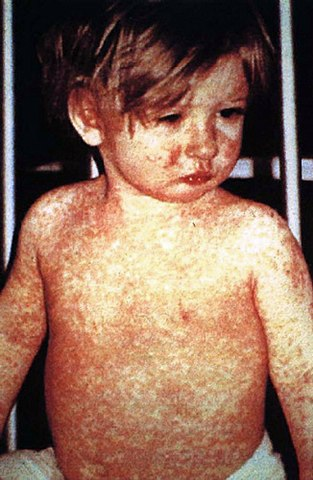
\includegraphics[width=0.3\linewidth]{160_rougeole}
  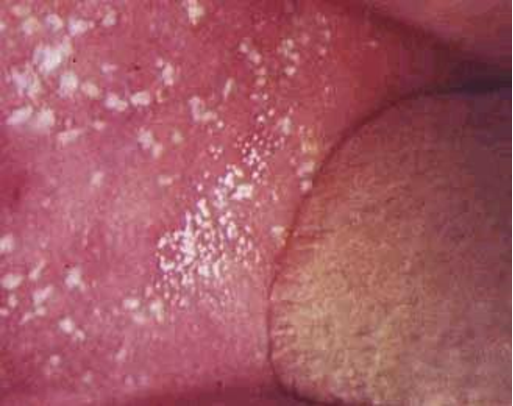
\includegraphics[width=0.5\linewidth]{160_rougeole_koplik.pdf}
\end{figure}

\begin{itemize}
\item
  très contagieux, contamination aérienne
\item
  diagnostic :~clinique++, NFS, PCR, sérologie

  \begin{itemize}
  \item
    catarrhe occulo-naso-bronchique fébrile
  \item
    signe de Köplick, exanthème maculopapuleux
  \end{itemize}
\item
  complications :

  \begin{itemize}
  \item
    respiratoires :~surinfections bactériennes (otites, laryngites,
    bronchites), pneumonies bactériennes/viral
  \item
    encéphalites : encéphalomyélite aigüe post-éruptive, encéphalite
    aigüe progressive, panencéphalite sclérosante subaigüe (PESS)
  \end{itemize}
\item
  traitement préventif : vaccin vivant atténué ROR (12M, 16-18M)
\end{itemize}

\begin{figure}
  \caption{Timeline: rougeole (gauche), rubéole (droite)}
\begin{tikzpicture}[
    every node/.style = {align=center},
    Line/.style = {-angle 90, shorten >=2pt},
    Brace/.style 2 args = { 
      semithick, decorate, 
      decoration={
        brace, #2,raise=2pt, 
        pre=moveto,pre length=2pt,
        post=moveto,post length=2pt,
        raise=#1,
      },
    },
    ys/.style = {yshift=#1}
  ]
  \linespread{0.8}                    
  \coordinate (a) at (0,0);
  % 2mm = 1j
  \coordinate[right=18mm of a]    (contag);
  \coordinate[right=32mm of a]    (incub);
  \coordinate[right=4mm of incub]    (invas);
  \coordinate[right=38mm of contag]    (contagFin);
  \coordinate[right=10mm of contagFin]    (fin);

  \draw[Line] (a) -- (fin) node[below left] {t};
  %\draw[Line] ([ys=9mm] invas) node[above] {Eruption} -- (invas);

  % Draw special brace
  \def\offset{10pt}
  \draw[Brace={\offset}{}] 
  (a) -- node [above=\offset] {Incubation (10-12j)} (incub);   
  \def\offset{35pt}
  \draw[Brace={\offset}{mirror}] 
  ( contag) -- node[below=\offset] {Contagiosité (10j)} ( contagFin);
  \def\offset{15pt}
  \draw[<->, transform canvas={yshift=-\offset}] 
  (incub) -- node[below] {Invasion (1-2j)} ( invas);
  \def\offset{10pt}
  \draw[Brace={\offset}{}] 
  (invas) -- node [above=\offset] {Eruption} (contagFin);   

  % draw vertical lines
  \foreach \x in {a, contag, incub, invas, contagFin} {
    \draw (\x) -- ([yshift=-1mm] \x);
  }
  \foreach \x/\y in {a/0, invas/14j, contagFin/19j} {
    \draw node at ([yshift=-3mm] \x) {\y};
  }

\end{tikzpicture}
\begin{tikzpicture}[
    every node/.style = {align=center},
    Line/.style = {-angle 90, shorten >=2pt},
    Brace/.style 2 args = { 
      semithick, decorate, 
      decoration={
        brace, #2,raise=2pt, 
        pre=moveto,pre length=2pt,
        post=moveto,post length=2pt,
        raise=#1,
      },
    },
    ys/.style = {yshift=#1}
  ]
  \linespread{0.8}                    
  \coordinate (a) at (0,0);
  % 2mm = 1j
  \coordinate[right=26mm of a]    (contag);
  \coordinate[right=32mm of a]    (incub);
  \coordinate[right=4mm of incub]    (invas);
  \coordinate[right=20mm of contag]    (contagFin);
  \coordinate[right=5mm of contagFin]    (fin);

  \draw[Line] (a) -- (fin) node[below left] {t};
  \draw[Line] ([ys=9mm] invas) node[above] {Eruption} -- (invas);

  % Draw special brace
  \def\offset{10pt}
  \draw[Brace={\offset}{}] 
  (a) -- node [above=\offset] {Incubation (16j)} (incub);   
  \def\offset{35pt}
  \draw[Brace={\offset}{mirror}] 
  ( contag) -- node[below=\offset] {Contagiosité (10-18j)} ( contagFin);
  \def\offset{15pt}
  \draw[<->, transform canvas={yshift=-\offset}] 
  (incub) -- node[below] {Invasion (1-2j)} ( invas);

  % draw vertical lines
  \foreach \x in {a, contag, incub, invas, contagFin} {
    \draw (\x) -- ([yshift=-1mm] \x);
  }
  \foreach \x/\y in {a/0, incub/16j} {
    \draw node at ([yshift=-3mm] \x) {\y};
  }

\end{tikzpicture}
\end{figure}


Mégalérythème épidémique

\begin{itemize}
\item
  contagion respiratoire
\item
  clinique : rash maculopapuleux (joue $\to$ tronc
  $\to$ extrémités), arthralgies
\item
  diagnostique : sérologie, PCR
\end{itemize}

Exanthème subit~:(HHV-6)?

\begin{itemize}
\item
  enfant 6 mois - 4 ans
\item
  clinique :

  \begin{itemize}
  \item
    fièvre 3-4 jours
  \item
    exanthème maculo-papuleux rose pâle + enanthème voile du palais
    (éruption 24h)
  \end{itemize}
\item
  traitement symptomatique
\item
  complications : celles de la fièvre
\end{itemize}

Autres exanthèmes :

\begin{itemize}
\item
  adénovirus
\item
  zika
\item
  VIH
\end{itemize}

\paragraph{Scarlatiniforme}

Scarlatine :
\danger angine + vomissements = scarlatine par défaut

\begin{itemize}
\item
  clinique :~

  \begin{itemize}
  \item
    début brutal (fièvre, céphalées, maux gorge, vomissements)
  \item
    exanthème se généralisant, marqués aux plis de flexion (8j)
    $\to$ desquamation
  \item
    enanthème orop-pharyngé-lingual (lange framboisée)
  \end{itemize}
\item
  traitement :~

  \begin{itemize}
  \item
    pénicilline V ou amoxicilline 10j
  \item
    antibioprophylaxie
  \end{itemize}
\end{itemize}

Syndrome de Kawasaki

\begin{itemize}
\item
  vascularite systémique aigüe
\item
  clinique :

  \begin{itemize}
  \item
    fièvre prolongée, exanthème, glossite
  \item
    adénopathies cervicales volumineuses
  \item
    desquamation en doigts de gants
  \end{itemize}
\item
  jeunes enfants
\item
  traitement : Ig IV 2j puis aspirine 14j {}
\end{itemize}

Sd du choc toxique

\begin{itemize}
\item
  Tampon périodique \textgreater{} 8h
\item
  Clinique : fièvre, état de choc, érythrodermie généralisée,
  desquamation tardive
\item
  traitement : clindamycine + gentamicine IV
\end{itemize}

\subsection{Virales vésiculeuses}

\paragraph{Vésiculeuses}

Varicelle : cf ~\nameref{subsec:varicelle}

Zona, Herpès : cf~\nameref{sec:item164}

Coxsackie : sd pieds-mains-bouche (vésicules ovalaires). Contagion par
les selles (10j). Clinique : vésicules fesses, pieds, bouche, lèvre

\paragraph{Pustuleuses} Poxviridae, variole

\subsection{Bulleux} Erythème polymorphe (lésion en cocarde). Toxidermies bulleuses :~sd de
Stevens-Johnson, sd de Lyell

\section{161 :~Oreillons}

Bénigne, contagieuse à réservoir humain. Diagnostic principalement
clinique :

\begin{itemize}
\item incubation 19j
\item invasion 24-48h
\item état : parotidite ourliennes (70\%) unilatérale puis bilatérale
\end{itemize}

Guérison spontanée 8-10j. Autres formes :

\begin{itemize}
\tightlist
\item
  neuroméningé++ : méningite lymphocytaire (pas de séquelles),
  encéphalite (décès 1-5\%, surdité possible)
\item
  orchite/épidymite ourlienne, atrophie testiculaire 50\%
\item
  pancréatie ourlienne : rare, guérison spontanée sans séquelle
\end{itemize}

Traitement symptomatique\\
Prévention :~vaccin ROR

\section{162 - Grippe}
\label{sec:item_162_grippe}

Transmission inter-humaine (gouttelettes)

\subsection{Diagnostic}%

\paragraph{Clinique}%
\label{par:clinique}

\danger Toux fébrile brutale novembre-févier en Europe \textit{ou} contact
grippe = grippe par défaut

\begin{figure}[htpb]
  \centering
\begin{tikzpicture}[
    every node/.style = {align=center},
    Line/.style = {-angle 90, shorten >=2pt},
    Brace/.style 2 args = { 
      semithick, decorate, 
      decoration={
        brace, #2,raise=2pt, 
        pre=moveto,pre length=2pt,
        post=moveto,post length=2pt,
        raise=#1,
      },
    },
    ys/.style = {yshift=#1}
  ]
  \linespread{0.8};
  \coordinate (a) at (0,0);
  % 2mm = 1j
  \coordinate[right=6mm of a]    (incub);
  \coordinate[right=4mm of a]    (contagDebut);
  \coordinate[right=14mm of incub]    (symptome);
  \coordinate[right=14mm of contagDebut]    (contagFin);
  \coordinate[right=10mm of contagFin]    (fin);

  \draw[Line] (a) -- (fin) node[below left] {t};

%  % Draw special brace
  \def\offset{10pt}
  \draw[Brace={\offset}{}] 
  (a) -- node [above=\offset] {Incubation (1-3j)} (incub);   
  \def\offset{30pt}
  \draw[Brace={\offset}]%{mirror}] 
  (incub) -- node[above=\offset] {Symptômes (7-15j)} (symptome);

  \def\offset{15pt}
  \draw[Brace={\offset}{mirror}] 
  (contagDebut) -- node[below=\offset] {Contagiosité 7j} (contagFin);

  % draw vertical lines
  \foreach \x in {a, incub, symptome} {
    \draw (\x) -- ([yshift=-1mm] \x);
  }
  %\foreach \x/\y in {a/0, incub/+7-21j}{%, quinte/+7-15j} {
    %\draw node at ([yshift=-3mm] \x) {\y};
  %}

\end{tikzpicture}
\end{figure}

Sd grippal :
\begin{itemize}
  \item 
    Local : ORL (rhinorrhée, pharyngolaryngite), trachéo-bronchique (toux sèche, irritative)
    \item Systémique : sd algique (céphalée, arthromyalgies, courbatures)
\end{itemize}

\paragraph{Complications}%
\label{par:complications}

\begin{itemize}
  \item respiratoires
    \begin{itemize}
      \item surinfection bactérienne : OMA, sinusite aigüe, surtout pneumonie aigüe =
        grippe maligne primaire (rare, $\skull$) et secondaire
    \end{itemize}
  \item extra-respiratoire
\end{itemize}

Examens microbiologie : seulement pour les grippes compliquées. Référence = PCR
Influenza

Hospitalisation : 
\begin{itemize}
  \item saisonnière : à risque, complications
  \item pandémie : forme grave/compliquée
\end{itemize}

\subsection{Traitement}%

Symptomatique.
Antigrippal = inhibiteurs de la neuramidase (oseltamivir, zanamivir)
\begin{itemize}
  \item curatif : < 48h !
  \item prophylaxie (pré- ou post-exposition)
\end{itemize}

\section{163 : Hépatites virales}

\begin{figure}[htpb]
  \begin{subfigure}{0.49\textwidth}
    \resizebox{\textwidth}{!}{
      \begin{tabular}{*{5}{c}}
        \toprule
        & Orofécale & Parentérale & Sexuelle & Maternofoetale\\
        \midrule
        A             & +         & (+)         & (+)      & \\
        B             &           & +           & +        & + \\
        C             &           & +           & (+)      & (+) \\
        D             &           & +           & (+)      & (+) \\
        E             & +         & (+)         &          & \\
        \bottomrule
      \end{tabular}
    }
    \caption{Transmission}
  \end{subfigure}
  \begin{subfigure}{0.49\textwidth}
    \resizebox{\textwidth}{!}{
      \begin{tabular}{*{5}{c}}
        \toprule
        & Guérison             & Fulminante          & Chronique \\
        \midrule
        A    & 100\%                & < 5\textperthousand & non\\
        B    & 90\% (adulte)        & 1\%                 & 10\% \\
        & 5\% (petite enfance) &                     & 95\% \\
        C    & 15-30\%              & Exceptionelle       & 70-85\% \\
        D    & si co-infection VHB  & 5\%                 & si surinfection\\
        E    & si IC                & < 5\textperthousand & si ID \\
        \bottomrule
      \end{tabular}
    }
    \caption{Évolution}
  \end{subfigure}
  \caption{Hépatites virales}
\end{figure}

\subsection{Diagnostic}%
Élévation transaminases $\pm$ clinique (asthénie, anorexie, hépatalgie)\\

\paragraph{Aigüe} \danger Y penser si fébrile aigüe + ictère/hypertransaminasémie

1ère intention : VHA, VHB.\\
Si négative : VHC si risque, VHE si zone tropicale ou porc, sd mononucléosique,
dengue/arboviroses si zone tropicale

\paragraph{Chronique} VHB, VHC si risque

\begin{table}[htpb]
  \centering
  \caption{Suivi}
  \label{tab:suivi}
  \begin{tabular}{*{4}{c}}
  \toprule
      & Aigüe                       & Chronique         & Guérison \\
  \midrule
  A   & Augmentation T.             & non               & normalisation T.\\
      & IgM                         &                   & \\
  \midrule
  B   & Augmentation T.             & Ag HBs+ > 6 mois, & normalisation T. \\
      & Ag HBs +, Ac anti-HBc +     & Ac anti-HBs-      & Ac anti-HBs+\\
      & IgM anti-HBc+, Ac anti HBs- &                   &\\
      & PCR élevée                  &                   & \\
  \midrule
  C   & Augmentation T.             &                   & normalisation T. \\
      & IgG anti-VHC+ \danger       & idem              & PCR neg.\\
      & PCR élevée                  & \\
  \midrule
  D   & Augmentation T.             &                   & PCR nég. \\
      & IgM                         & IgG               & \\
  \midrule
 E    & Augmentation T. ?           & idem              & normalisation T. \\
      & IgM                         &                   & PCR neg.\\
  \bottomrule
  \end{tabular}
\end{table}

\subsection{Prise en charge}
Symptomatique : pas de paracétamol, AINS, alcool

Urgence = hépatite fulminante \skull : sd hémorragique + signes d'encéphalite
(confusion, inversion rythme nycthéméral, somnolence, astérixis)

\paragraph{VHB+VHC} bilan biologique, histologique (sauf cirrhose évidente)
directe (score METAVIR) ou indirecte, imagerie (échographie abdo puis IRM),
fibro (varices oeosphage/cardia)

\paragraph{VHB} Interférons pégylée $\alpha{}2a$, $\alpha{}2b$ (tolérance
médiocre), analogue nucléosidique (entécavir [toxicité musculaire]), nucléotidique (ténéfovir
[tox. rénale].

\paragraph{VHC} si fibrose $\ge F2$, manif. extra-hépatique. Ribavirine ou
antiviraux d'action directe (++).

\subsection{Prévention}
Hygiène, vaccination VHA (autour d'un cas), VHB

\section{164 - Infections à herpès virus du sujet immunocompétent}
\label{sec:item164}

Herpesvirinae

\begin{itemize}
\tightlist
\item
  Alpha- : HSV1 et 2, VZV
\item
  Beta : CMV, HHV-6 (roséole), HHV-7
\item
  Gamma- :~EBV (MNI), HHV-8 (sarcome de Kaposi)
\end{itemize}

Primo-infection puis latente à vie (récurrence)

\begin{table}[htpb]
  \centering
  \begin{tabular}{*{4}{c}}
    \toprule
    & & Immunocompétent& Immunodéprimé\\
    \midrule
    \multirow{2}{*}{Aciclovir IV} & HSV & 
        \begin{tabular}{c}
        grave : méningoencéphalite,\\~oculaire sévère,
        \\gingivostomatite sévère
      \end{tabular}&primo-infection, réactivation\\
    & VZV& grave : encéphalite, pneumopathie& varicelle, zona\\
    \midrule
    \multirowcell{2}{ Valaciclovir PO,\\Famciclovir PO} & HSV & 
        \begin{tabular}{c}
          génital, cutanéomuqueux,\\oculaire non sérèves
        \end{tabular} & \\
    & VZV& 
    \begin{tabular}{c}
      ophtalmique,risque d'algie\\post-zostérienne
    \end{tabular}&\\
    \bottomrule
  \end{tabular}
\end{table}


\begin{table}[htpb]
  \centering
  \caption{Traitement HSV}
  \begin{tabular}{*{4}{c}}
    \toprule
    & & Immunocompétent& Immunodéprimé\\
    \midrule
    Aciclovir IV& HSV& 
    \begin{tabular}{c}
      grave : méningoencéphalite,\\~oculaire sévère,
      \\gingivostomatite sévère
    \end{tabular}&primo-infection, réactivation\\

    & VZV& grave : encéphalite, pneumopathie& varicelle, zona\\
    \midrule
    \begin{tabular}{c}Valaciclovir PO,\\Famciclovir PO
    \end{tabular}& HSV& 
    \begin{tabular}{c}
      génital, cutanéomuqueux,\\oculaire non sérèves
    \end{tabular}
    & \\
    & VZV& 
    \begin{tabular}{c}
      ophtalmique,risque d'algie\\post-zostérienne
    \end{tabular}&\\
    \bottomrule
  \end{tabular}
\end{table}

\subsection{CMV}

Transmission par contact direct Immunodéprimé :~greffe de CSH,
transplantation d'organe, SIDA

\subsection{EBV}

Contamination salivaire. Primo infection = VCA IgG +/- \footnote{viral capsid antigen}
, VCA Ig +, EBNA IgG-\footnote{Epstein Barr Nuclear Antigen}

Contexte: MNI, allogreffe CSH, VIH

\subsection{HSV1, 2}

Transmission :~directe, cutanéomuqueuse, transplacentaire

\begin{table}[htpb]
  \centering
  \begin{tabular}{*{4}{c}}
    \toprule
    Type& Localisation& Primo& Récurrence\\
    \midrule
    HSV1& plutôt orale& 
      \begin{tabular}{c}
        enfance,~asymptomatique\\
        (ou gingivostomatite aigüe)
      \end{tabular} &
      \begin{tabular}{c}
        Vésicules unilatérales\\(narines, menton).\\
        Kératite possible
      \end{tabular}
    \\
    \midrule
    HSV2& plutôt génitale& 
      \begin{tabular}{c}
        Érythémato-vésiculeuses\\+ exsudat blanchâtre
      \end{tabular} &
      \begin{tabular}{c}
        Prodromes puis\\~Lésions :~vésicules,\\guérison 7-10j
      \end{tabular}\\
    \bottomrule
  \end{tabular}
\end{table}

Traitement :\\

\begin{itemize}
  \item gingivostomatite aigüe : spontanément favorable 
  \item ophtalmologique :~aciclovir pommade (+ IV ?), pas de corticothérapie \danger 
  \item  préventif si > 6 récurrences/an (valaciclovir quotidien 6-12 mois)
\end{itemize}

\subsection{Varicelle}
\label{subsec:varicelle}
90\% chez l'enfant, plus grave chez l'adulte Diagnostique clinique

\begin{itemize}
\tightlist
\item
  incubation (14j)
\item
  état : (maculo-papule) $\to$ vésicules (prurit+++)
  $\to$\_érosion + pseudo-ombilication $\to$ croûtes
  (J4) $\to$ cicatrisation (J10)
\item
  spontanément favorable (10-15j)
\end{itemize}

Complications :

\begin{itemize}
\item surinfection bactérienne fréquente (grattage)
\item terrains, état infectieux sévère, respiratoie neuro, purpura
  thrombopénique aigu
\end{itemize}

Traitement :

\begin{itemize}
\item symptomatique (pas d'aspirine, ni AINS ⚠)
\item ATB si surinfection cutanée, antiviral si formes graves/compliquées
\item pas d'éviction scolaire
\item vaccination : ado, \female en âge de procréer, contact avec ID, professionnel.
  \skull pas la femme enceinte !
\end{itemize}

NB : toxicité rénale pour l'aciclovir

\subsection{Zona}

Réactivation du VZV. Gravité : douleurs post-zostériennes,
immunodépression, localisations

Diagnostic : clinique

\begin{itemize}
\item prodrome
\item état :~éruption (érythémateux roses vifs $\to$ vésicules en
  bouquets $\to$ érosives $\to$ croûtes
  $\to$ cicatrices dépigmentées (rosées $\to$
  blanchâtres) + fébricule
\item poussées sur 2-3 semaines, douleurs plusieurs mois
\end{itemize}

Complications : principalement DPZ (rarement neurologique)

Traitement

\begin{itemize}
\item local : symptomatique, douleur (antalgique phase aigüe)
\item ATB si surinfection cutanée, antiviral en prévention DPZ (valaciclovir
  per os 7 jours)
\item prévention vaccination (entre 65 et 74 ans)
\end{itemize}

\subsection{Complications}

HSV1, 2 :

\begin{itemize}
\item nouveau-né (périnatale++) :~mortalité très élevée, séquelle
très lourdes 
\item femme enceinte : maladie chez nouveau-né 
\item atopique : Kaposi-Juliusberg VZV
\end{itemize}

\section{165 - VIH}

Transmission : sexuel, sang, mère $\to$ enfant Prévention
:~TasP (Treat as Prevention), TPE (Traitement Post-Exposition),
traitement pré-exposition, prévention de la transmission mère-enfat

\subsection{Sérologie}

\begin{figure}[htpb]
  \centering
  \caption{Fenêtre diagnostique}
  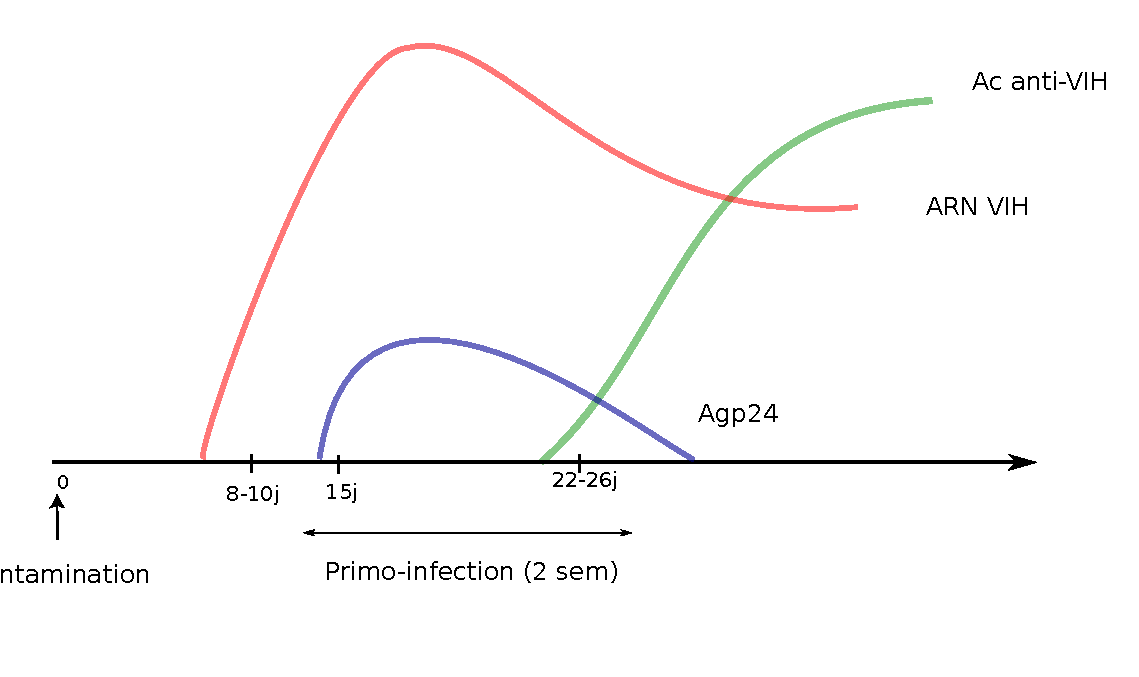
\includegraphics[width=0.8\linewidth]{165_diag}
\end{figure}

Tests diagnostics

\def\mminus{\large\textbf{-}}
\def\pplus{\large\textbf{+}}

\begin{figure}[htpb]
  \centering
\tikz \graph [
  % Labels at the middle 
  edge quotes mid,
  % Needed for multi-lines
  nodes={align=center},
  level distance=2cm,
  %sibling distance=3cm,
  edges={nodes={fill=white}}, 
layered layout]
{
  "Elisa (Ac, Ag p24)" -> {
    "> 6 semaines ?" [>"\mminus"] -> {
      "Elisa (2eme)" [>"non"];
    };
    "Western-Blot" [>"\pplus"] -> {
      "Elisa" [>"\pplus"];
    };
  };
};
\end{figure}

\begin{table}[htpb]
  \centering
  \begin{tabular}{cc}
    \toprule
    Infection non-opportuniste& Prévention\\
    \midrule
    Pneumonie à S. pneumonia& Vaccin\\
    Infections digestions& Hygiène alimentaire\\
    Grippe& Vaccin\\
    IST (syphilis, gonococcies, C. trachomatis, HPV)& Préservatif, dépistage, vaccin VHA, VHB (homosexuel hommes)\\
    VHB, VHC& Surveillance, vaccination\\
    \bottomrule
  \end{tabular}
\end{table}

\begin{table}[htpb]
  \centering
  \begin{tabular}{cccc}
    \toprule
    Infection opportuniste& Seuil CD4& Diagnostic& Prévention\\
    \midrule
    Tuberculose  & $\emptyset$ & BK, anatomopath. & ITL par IGRA\\
    Candidose oesophagienne  &< 200& Clinique& $\emptyset$\\
    Pneumocystose pulmonaire  &< 200& Radio thorax, prelev.  respi& CTM si CD4 < 200\\
    Toxoplasmose cérébrale  &< 200& TDM/IRM $\to$ sérologie $\to$ PCR LCS \\
    && $\to$ test thérapeutique $\to$ biopsie& CTM (CD4 $\to$ 100)\\
    CMV  & < 100& PCR& \danger rétinite\\
    Cryptococcose& < 100& LCS& \\
    LEMP& < 100& IRM, PCR LCS& \\
    Mycobactérioses atypiques& < 100& Hémocultures, prélèvement& \\
    \bottomrule
  \end{tabular}
  \caption{VIH : infecions opportunistes. BK=bacille de Koch, CMT =
  Cotrimoxazole. Mnémo: "quand les pneus sont toxiques" pour < 200}
\end{table}

🔥 = fréquents

\begin{longtable}[]{@{}ll@{}}
\toprule
Cancers classant SIDA & Cancers non classants\tabularnewline
\midrule
\endhead
Lymphome malin non hodgkinien & Cancer du canal anal\tabularnewline
Maladie de Kaposi & Hépatocarcinome\tabularnewline
Cancer du col de l'utérus &\tabularnewline
\bottomrule
\end{longtable}

\subsection{Traitement}

Toxicité long-terme : lipodystrophie, CV, rénale, osseuse, métabolique

\begin{figure}[htpb]
  \centering
\tikz \graph [
  % Labels at the middle 
  edge quotes mid,
  % Needed for multi-lines
  nodes={align=center},
  %sibling distance=3cm,
  edges={nodes={fill=white}}, 
layered layout]
{
  "\textbf{2 inhibiteurs nucléosidiques de la transcriptase inverse}\\
  Abacavir + lamivudine 
  ou ténéfovir + emtricitabine" -> {
    "\textbf{1 INNTI}\\Rilpivirine";
    "\textbf{1 inhibiteur de la protéase}\\Darunavir";
    "\textbf{1 inhibiteur de l'intégrase}\\Dolutégravir/Raltégravir/Elvitégravir";
  }
};
\end{figure}

\subsection{Vaccins}

Grippe, fièvre jaune, tétanos, diphtérie, VHB, VHA, HPV, pneumocoque


\section{166 - Paludisme}

Fièvre + retour zone d'endémie palustre = paludisme par défaut


Géographie
\begin{figure}[htpb]
  \centering
  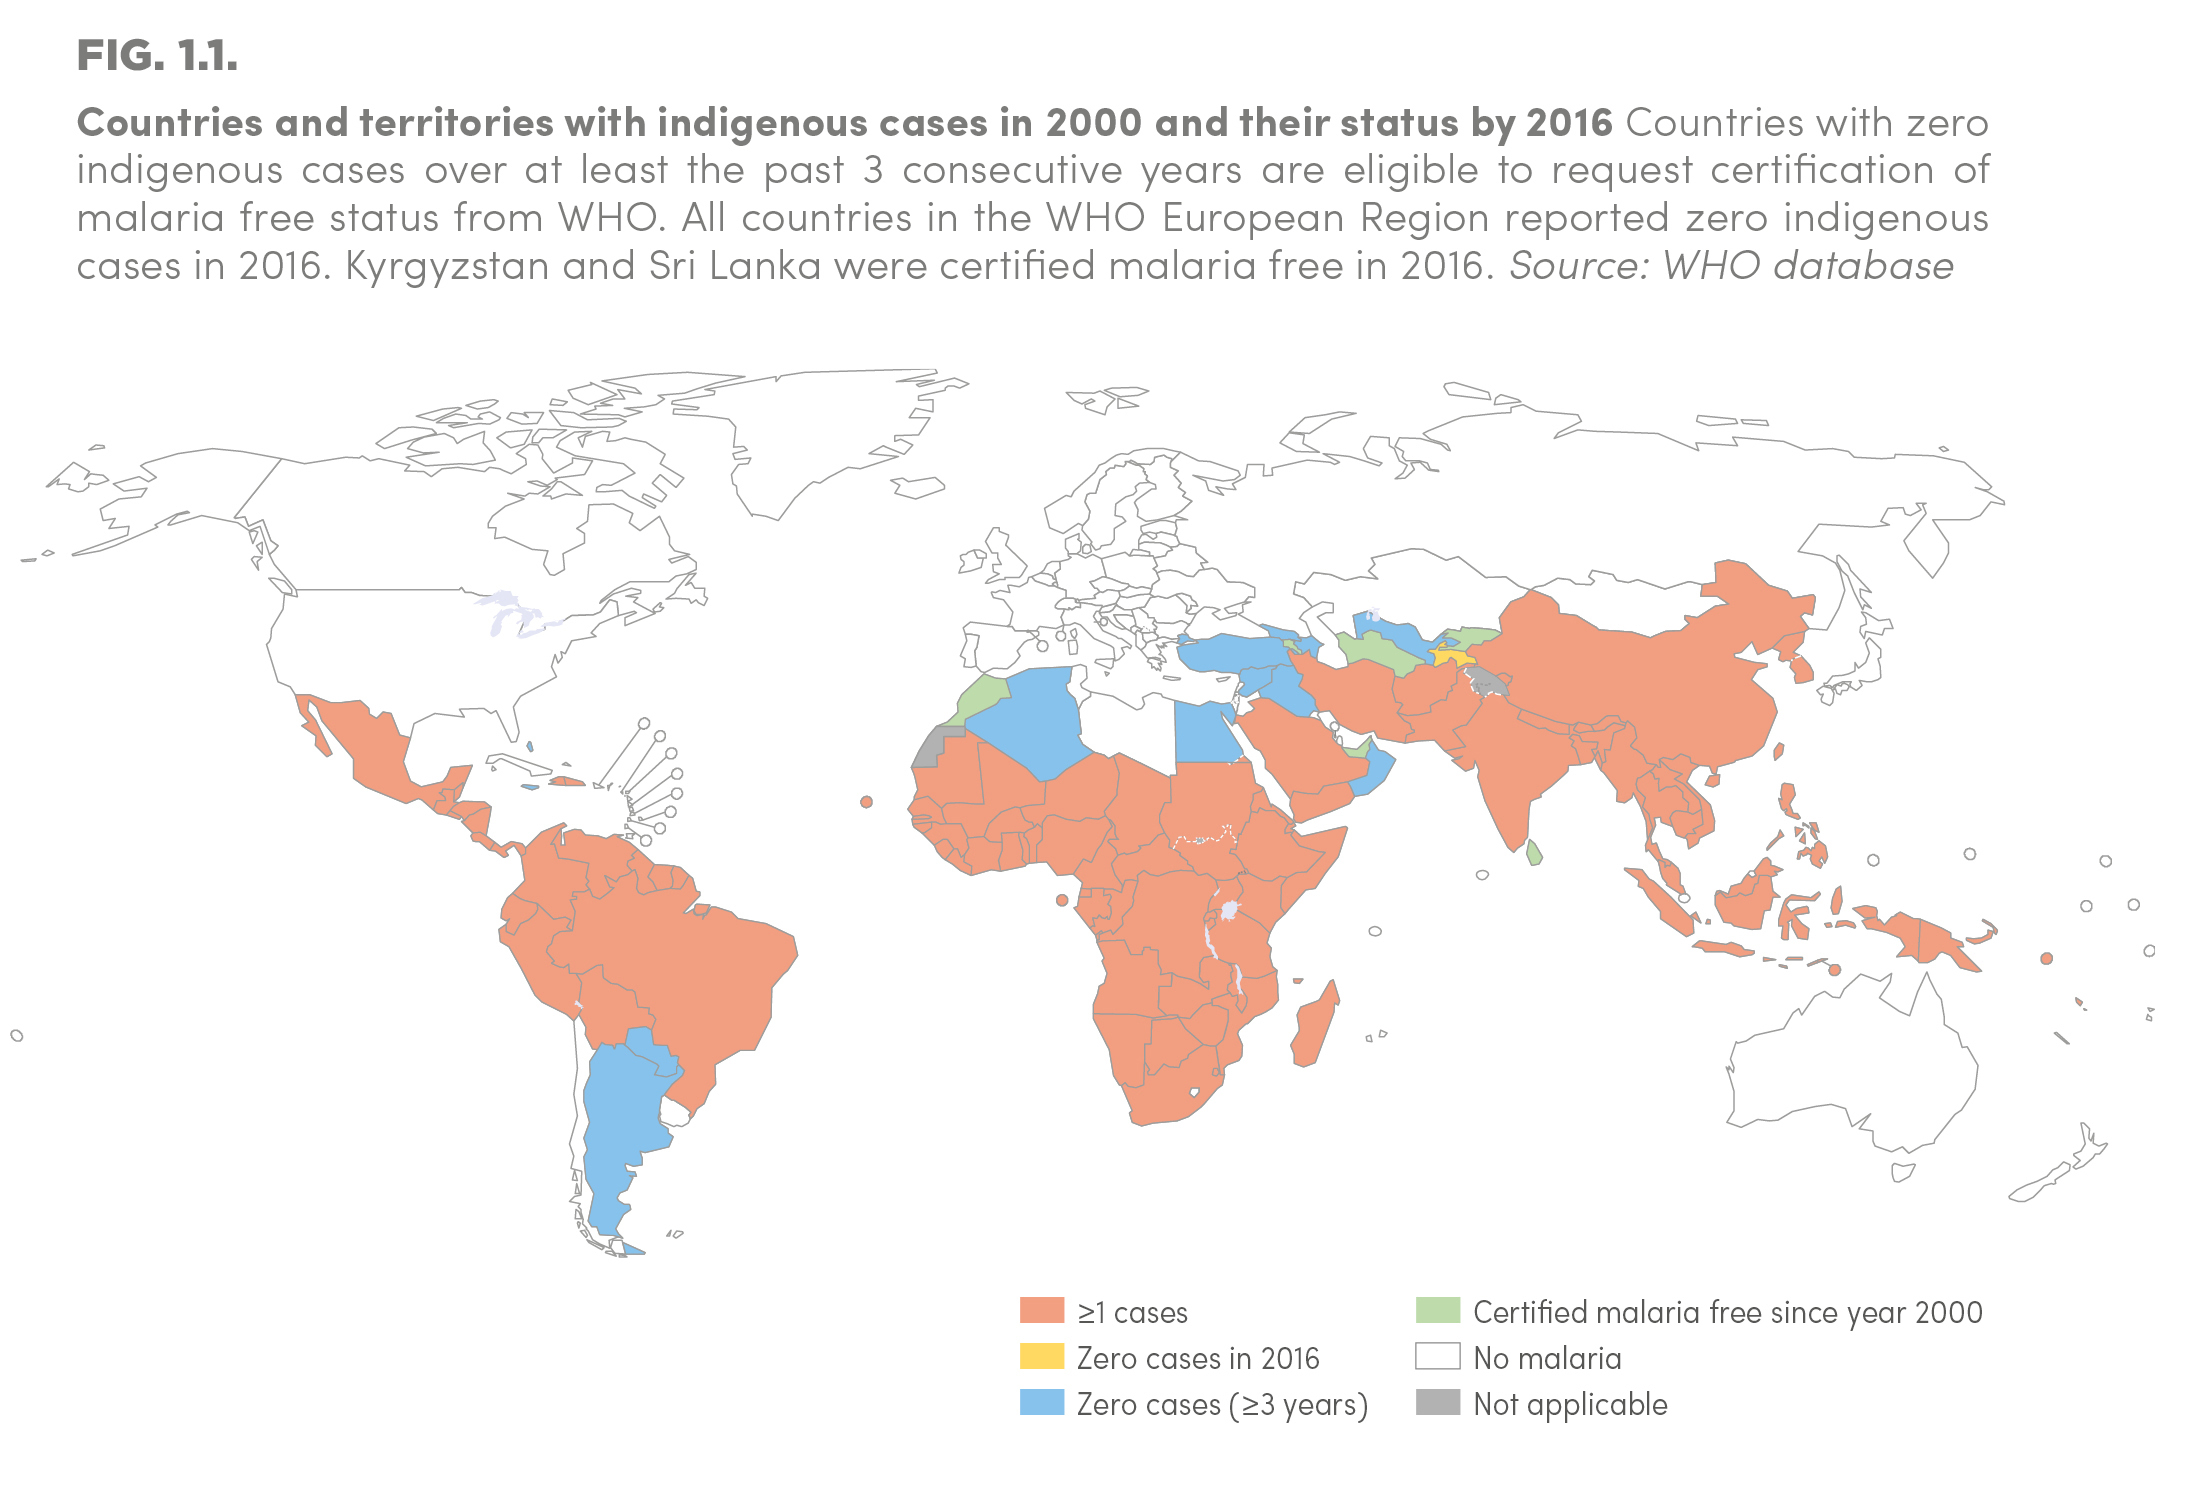
\includegraphics[width=0.8\linewidth]{palu_map_2016.jpg}
\end{figure}

Démarche

\begin{figure}[htpb]
  \centering
\tikz \graph [
  % Labels at the middle 
  edge quotes mid,
  % Needed for multi-lines
  nodes={align=center},
  %sibling distance=3cm,
  edges={nodes={fill=white}}, 
layered layout]
{
  "Fièvre\\
  Céphalée, myalgies\\
  Troubles digestif\\
  (Splénomégalie)"
  ->
  "Frottis sanguin\\
  +goutte épaisse\\
  +/- Ag circulants" [draw] -> {
    "P. vivax/ovale\\/malariae" -> "Chroloquine PO" [draw];
    "P. falciparum\\/knowlesi" -> {
      "Signes de gravité ?" [level distance=40pt] -> ["oui"] "\faHospitalO{} urgence\\artésunate IV" [draw];
      "Signes de gravité ?" ->["non"] "\faAmbulance{} possible ?" -> "Vomissements ?" 
          };
  };
  "Vomissements ?" [level distance=50pt] -> {
    "Quinine IV" [>"oui", draw];
    "Dihydroartémisinine\\-pipéraquine PO\\
    \textit{ou} artéméther\\-luméfantrine PO" [>"non", draw];
  };

};
\end{figure}

\begin{table}[htpb]
  \centering
  \caption{Signes de gravité du paludisme}
  \begin{tabular}{cc}
    \toprule
    Critère& Seuil\\
    \midrule
    Défaillance neuro& \\
    Défaillance respi& Ventilé:~\(PaO_2/FiO_2 < 300\) mmHg\\
    & Non ventilé : \(PaO_2 < 60\) mmHg\\
    & ou \(SpO_2 < 92\) \% ou FR > 30/min. \\
    &Radio (interstitelle, alvéolaire)\\
    Défaillance CV& PA systol. < 80 mmHg + signes insuffisance circulatoire\\
    Hémorragie& clinique\\
    Ictère& clinique / bilirubine \(> 50 \mu{}mol/L\)\\
    Hémoglobuinurie macroscopique& \\
    Anémie& Hg < 5 g/dL, Ht < 20\%\\
    Hyoglycémie& glycémie < 2.2 mmol/L\\
    Acidose& bicarbonates plasma. < 15 mmol/L ou ph < 7.35\\
    Hyperlactémie& > 2 mmol/L\\
    Hyperparasitémie& > 4\%\\
    Insuffisance rénale& créat. \(> 65 \mu{}mol/L\) ou urée sanguine > 20 mmol/L\\
    \bottomrule
  \end{tabular}
\end{table}

\section{167 - Gale et pédiculose}

Ectoparasitoses humaines strictes, très contagieuses. Prurit++

\subsection{Gale}
\paragraph{Clinique} 5j-1mois incubation.\\
Prurit avec contage, collectif, nocturne, pas sur le dos ni visage\\
Sillons épidermiques, vésicules perslé, nodules scabieux, lésions de grattage

Diagnostic : paralistologique (visuel ou grattage). Penser IST

\paragraph{Traitement} 
Indivuel et collectif\\
Ivermectine 1ere intention (> 15kg) ou benzoate de benzyle\\
Traitement linge, précautions contact, surinfection bactérienne

\subsection{Pédiculose}
Porteur de \bact{typhus}, \bact{tranchees}, \bact{recurrente}

\begin{itemize}
  \item Corporelle : précarité. Clinique=dos, thorax. Ttt = vêtements, literie
    \item Cuir chevelu : enfants. Clinique = prurit diurne, nocturne sur
      cheveux. Lentes visibles. Ttt = malathion ou dimeticone. Décontamination
      \item Pubien : clinique = lésions de gratage. Déister IST !. Ttt = pyréthrinoïde
\end{itemize}

\section{168 - Parasitoses digestives}
Protozoaires (unicellulaires) : amoebose, giardiose\\
Helmintes (pluricellulaires) : 
\begin{itemize}
  \item plathelminthes = téniasis, cysticercose, hydatidose, 
  \item nemathelminthes = asciridiose, oxyurose
\end{itemize}
Traitement : métronidazole pour protozoaires, albendazole pour helmintes\\
En france : giardiose, oxyurose\\
Transmission féco-orale sauf téniasis

\paragraph{Giardiose} Formes : végétatives/kystique. \\
Souvent asymptomatique. EPS (biopsie jéjunale si végétative)\\
Controle EPS. Hygiène

\paragraph{Téniasis} \bact{saginata} (boeuf) et \bact{solium} (porc).\\
  Adulte ou cysticercose (enkystement)\\
  Diagnostic = 
  \begin{itemize}
    \item adultes : anneaux dans les selles, EPS
    \item cysticercose : épidémio, scanner, calcifications musculaires
  \end{itemize}

\paragraph{Ascaridiose} fréquent pays en développement. Souvent asymptomatique.
Diagnostic : EPS

\paragraph{Oxyurose} Asymptomatique, prurit anal nocture. Diagnostic : oeil nu,
scotch test. Contrôle par EPS

\paragraph{Amoebose} 
\begin{itemize}
  \item intestinale aigüe : diag = pas de fièvre, sd dysentérique (subaigüe
    souvent). 3 EPS. Rectoscopie éventuelle : ulcérations en "boutons de chemise"
  \item hépatique : diag = fièvre, douleur hypochondre droit, hépatomégalie.
    Radio, échographie éhaptique. Sérologie Ac anti-amibiens
\end{itemize}

\section{169 - Zoonoses}%
\label{sec:ue_6_169_zoonoses}

\paragraph{Pasteurellose} morsure, griffure animale/végétale
Clinique: inflammation majeure en 3-6h autour de la plaie\\
Diagnostic : prélèvement plaie -> culture\\
Traitement: amoxicilline

\paragraph{Maladie des griffes de chat} Griffure de chat (jeune)\\
Clinique : locorégionale + au moins une adénobathie. 2-3 semaines incubation
Endocardite à hémoc. négatives\\
Diagnostic : sérologie (PCR si doute)\\
Traitement : si systémique et viscérale, azithromycine

\paragraph{Maladie de Lyme} Piqûre de tique\\
Clinique :
\begin{itemize}
  \item primaire : érythème migrant $\pm$ signes généraux
  \item secondaire : 
    \begin{itemize}
      \item neurologique = ménigoradiculite (sensitif, liquide clair
        lymphocytaire, normoglyco, hyperprot), méningite, encéphalite/myélite
      \item articulaire = oligoarthrite sur grosses articulaires
      \item cardiaque = myocardite (ECG ?)
      \item cutanée = lymphocytome borrélien
      \item oculaires 
    \end{itemize}
  \item tertaire : cutanées (acrodermatite chronique atrophiante = quasi
    pathognomonique), neurologique, articulaires
\end{itemize}
Diagnostic : 
\begin{itemize}
  \item érythème migrant
  \item OU clinique + épidémio + sérologique (Elisa + WB) + pas de DD
\end{itemize}
Traitement : amoxicilline/doxycycline (primaire), ceftriaxone/doxycycline
(secondaire/tertaire)

\paragraph{Fièvre Q} Digestive ou inhalation\\
Clinique : 
\begin{itemize}
  \item aigüe : hépatite fébrile/pneumopathie/fièvre isolée. 3 semaines d'incubation
  \item chronique : endocardite infectieuse à hémoc. négatives
\end{itemize}
Diagnostic : sérologie\\
Traitement : doxycycline


\paragraph{Tularémie} Contact lagomorphes/piqûre de tique\\
Clinique : après 4 j, fièvre + adénopathies inflammatoires (satellites lésions)
Diagnostic : Sérologie + PCR\\
Traitement : doxycycline


\paragraph{Rickettsioses} 
\begin{itemize}
  \item \bact{conorii} : tiques du chien. Clinique : fièvre + tâche noire +
    éruption maculo-papuleuse
  \item \bact{typhus} poux du corps. Clinique : fièvre + éruption
    maculo-papuleuse
\end{itemize}
Diagnostic : sérologie + PCR\\
Traitement : doxycycline

\paragraph{Brucellose} Contaminations à l'étranger (ruminant/porcins)\\
Clinique :
\begin{itemize}
  \item aigüe : fièvre ondulante sudoro-algique, arthromyalgie, adénopathies,
    hépatosplénomégalie
  \item subaigüe/chronique
\end{itemize}
Diagnostic : sérologie (+ hémoc. si aigüe)\\
Traitement : doxycycline + gentamicine/rifampicine

\paragraph{Toxoplasmose} Alimentation\\
Clinique : asthénie, fièvre modérée, polyadénopathie. Si ID : kyste
cérébraux/oculaires\\
Diagnostic : infection aigüe, sérologie, PCR\\
Traitement : aucun, évolution bénigne. Femme enceinte : spiramycine. ID :
pyriméthamine + acide folinique + sulfadiazine

\paragraph{Leishmaniose} Piqûre de phléobotome (nuit), zones tropicales
\begin{itemize}
  \item forme cutanée : lésion. 
  \item forme viscérale : fièvre hectique, anémie, amaigrissement,
    hépatosplénomégalie, adénopathies.
\end{itemize}
Diagnostic : ED, culture, PCR (sérologie si viscérale)\\
Traitement : cutané (local), amphotéricine B liposomale (viscérale)

\paragraph{Hydatidose (échinococcose hydatique)} Contact chien/aliments
souillés.
Clinique : asymptomatique\\
Diagnostic : sérologie.\\
Traitement : pas de ponction-biopsie du kyste \danger. Chir + albendazole

\paragraph{Rage} 
Risque élevée (chauve-souris, zone de rage, animal porteur): vaccination
curative + sérothérapie\\
Risque quasi-nul : rien\\
risque non nul : vaccination curative
 
\section{170 - Pathologies chez les migrants}%
\label{sec:ue_6_170_pathologies_chez_les_migrants}
\subsection{Diagnostic}

\begin{table}[htpb]
  \centering
  \caption{Risque majeur suivant la géographie}
  \begin{tabular}{*{5}{c}}
  \toprule
               & Afrique subsaharienne & Afrique du N & Asie SE & Amérique latine \\
  \midrule
 Tuberculose   & X                     & X            & X\\
    VHB
               & X                     & X            & X\\
 VIH           & X \\
 Téniasis      & X                     & X            & X\\
 Bilhariozes   & X \\
 Paludisme     & X                     &              & X \\
 Hydatidose    &                       & X            &         & X\\
 Gale          & X                     & X            & X       & X \\
  \bottomrule
  \end{tabular}
\end{table}

\paragraph{Étiologies} 
Parasitose
\begin{itemize}
  \item paludisme (fièvre + zone endémie)
  \item parasitoses amoebiose, giardiose, ascaridiose, ankylostomose,
    anguillolose [dépistage si immunosuppresseur], hydatidose, tédiasis
    [penser neurcysticercose si comitialité]
  \item filariose : loase, filarioses lymphatiques, (onchocercose)
  \item schistosomoses
  \item leishmanioses
  \item trypanasomoses africhaine, américaine
  \item gale
\end{itemize}
Mycoses : dermatophyties (histoplasmoses)\\
Bactéries : tuberculose + VIH, lépre\\
Viral : VIH\\

\subsection{Protection maladie}
Aide Medicale del'Etat : $\ge 3$ mois + pas titre séjour + faibles ressources \\
Couverture Maladie Universelle : régulière $\ge 3$ mois 

\subsection{Préventions}
\danger Penser paludisme en premier\\
Vaccins : méningocoque (La Mecque), {VHA, VHB, typhoïde (fièvre jaune)} si
retour au pays

\section{171 - Voyage en pays tropical}%
\subsection{Vaccins}%
Routine : DTP, coqueluche, rougeole, VHB, BCG (enfant), grippe (> 65 ans)\\
Obligatoire : fièvre jaune (Amazonie, Afrique intertropicale), méningocoque
(Arabie Saoudite)\\
Recommandés :
\begin{itemize}
  \item VHA : bas niveau d'hygiène
  \item typhoïde : prolongé (Inde)
  \item cholérique : personnel médical + épidémie
  \item rage: prolongé + risque
  \item méningite ("ceinture" africain)
  \item encéphalite japonaise
  \item encéphalite tiques (Europe central, Est, Nord)
\end{itemize}

\subsection{Fièvre, diarrhée, lésions cutanées}
\begin{table}[htpb]
  \centering
  \caption{Fièvre}
  \begin{tabular}{*{4}{c}}
  \toprule
  Durée        & Étiologie           & Clinique                & Confirmation \\
  \midrule
  < 7 j        & dengue, chikungunka & Myalgies, arthralgie    & PCR (< 5 j)\\
               &                     & Rash J3-J5              & Sérologie sinon\\
  \midrule
  < 2 semaines & typhoide            & Céphalées++, SMG        & Hémocultures\\
               & rickettsioses       & &\\
  \midrule
  1sem - 2 mois& paludisme          & Digestif, neuro, SMG     & Frottis/goutte épaisse\\
  > 10j        & hépatites virales  & Digestif, ictère        & Sérologies \\
  mois/années  & amoebose hépatique & HMG douloureuse, fièvre & écho foie $\pm$ TDM\\
               &                    &                         & Sérologie\\
  2-6 sem      & schistosomose      & Prurit, arthralgie, HMG & Sérologie, EPS\\
  \bottomrule
  \end{tabular}
\end{table}

Diarrhée :
\begin{itemize}
  \item fébrile : paludisme puis shigellose, salmonelle, Campylobacter
    $\rightarrow$ coproculture
  \item sinon parasitaire $\rightarrow$ EPS. Giardose = + fréquente
\end{itemize}

Lésions cutanées : 
\begin{itemize}
  \item fréquent = pyodermites \bact{dore}/\bact{pyogenes}
  \item escarre : rickettsiose
  \item exanthème fébrile : arbovirose, leptospirose, syphilis, VIH,
    rickettsiose, médicament
  \item urticaire : schistosomose, hépatite virale, rickettsiose, médicament
\end{itemize} 

Typhoïde : \bact{salmonelle} (para)typhi. Hémocultures $\pm$ coproculture. ATB :
C3G parentéral (proba) puis documenté (FQ). Vaccin disponible (60\%)

\vspace{10pt}
Arboviroses : transmission arthropode. Guérison 7eme jour ou
hémorragie/encéphalite. PCR puis sérologie
\begin{itemize}
  \item dengue = 2eme cause fièvre tropicale
  \item chikungunya : dengue-like + arthralgie persistante
  \item fièvre jaune
  \item zika : généralement bénin
  \item encéphalite
\end{itemize}

\section{172 - Diarrhées infectieuses}%
\label{sec:ue_6_172_diarrhees_infectieuses}

\begin{table}[htpb]
  \centering
  \caption{Étiologies infectieuses des diarrhées aigües}
  \begin{tabular}{ccc}
  \toprule
                       & Syndrome cholériforme        & Entéro-invasif\\
  \midrule
                       & Virus                        & Shigelloses \\
                       &                              & Salmonelloses non typhi \\
                       &                              & Campylobacter \\
                       &                              & Yersinia \\
                       &                              & E. coli entéropathogène\\
   \midrule
   Diarrhée post-ATB   &                              & \bact{difficile}\\
   \midrule
   TIAC                & \bact{dore}                  & Salmonelloses mineures\\
                       & \bact{cereus}                & Shigelloses\\
                       & \bact{perfringens}           & \bact{jejuni}\\
                       &                              & \bact{ecoli} entéro-hémorr./aggr.\\
   \midrule
    Voyage             & Virus                        & Amoebose colique \\
                       & Cryptosporidies  \\
                       & \bact{ecoli} entérotoxin. \\
                       & Choléra\\
  \bottomrule
  \end{tabular}
\end{table}

\bigskip
\danger Urgences : Déshydratation, sepsis gravie, sd pseudo-occlusif, diarrhée fébrile + retour
endémie \skull

\subsection{Examens}
Coproculture : si diarrhée aigüe/TIAC fébrile $\rightarrow$ SSYC
Recherche virus\\
EPS \\
Toxine \bact{difficile}\\
Hémoc si fièvre

\subsection{Traitement}
FQ ou azithromycine + symptomatique

\subsection{TIAC}

\begin{table}[htpb]
  \centering
  \caption{Causes de TIAC}
  \begin{tabular}{ccc}
  \toprule
   Agent                        & Incubation & Clinique\\
  \midrule
    \bact{dore}                 & 2-4h       & vomissements, douleurs abdo\\
                                &            & diarrhé, pas de fièvre\\
    \bact{perfringens}          & 8-24h      & Diarrhée sans fièvre\\
    \bact{salmonelle} no typhi  & 12-24h     & Diarrhée aigüe fébrile\\
    Noroviris                   & 24-48h     & idem \bact{dore}\\
  \bottomrule
  \end{tabular}
\end{table}

\section{173 - Prescription des antibiotiques}

\begin{table}[htpb]
  \hspace*{-3cm}
  %\centering
  \caption{Pénicillines}
  \begin{tabular}{*{5}{c}}
  \toprule
  Peni. G/V                    & Amoxicilline         & Amox. + inhib $\beta$ &
                                                                                Péni. M & Carboxy\\
                               &                      &  & /uréïdo-peni.\\
  \midrule
  Streptocoques                & Idem peni G+         & Idem amox + & Staph.  meti-S & idem amox + \\
  \bact{diphterie}             & Pneumocoques péni-S  & Staph. meti-S & & bacilles G- \\
  Fusobacterium                & \bact{faecalis}      & \bact{influenzae}\\
  Treponema                    & \bact{listeria}      & \bact{catarrhalis} \\
                               & \bact{meningocoque}  & \bact{ecoli} et autres entérobact. \\
                               & Borrelia             & produisant pénicillinase\\
                               & Entérobactérie grp I & Baccilles G- anaérobies\\
  \midrule
  \multicolumn{2}{c}{Réactions allergiques}\\
  \bottomrule
  \end{tabular}
\end{table}

\begin{table}[htpb]
  \centering
  \caption{Céphalosporines}
  \begin{tabular}{*{3}{c}}
  \toprule
  C2G                      & C3G orales            & C3G IV\\
  \midrule
  Cocci G+                 & Idem C2G +            & Ceftriaxone, cefotaxime : strept.\\
  (strepto, staph. méti-S) & Entérobactérie grp II & Neisseria, entérobact, Haemophilus\\
  Entérobactérie grp I     &                       & Ceftazidime, céfépime : \\
                           &                       & \bact{aeruginosa} \\
  \midrule
  \multicolumn{2}{c}{Allergies cutanées}\\
  \bottomrule
  \end{tabular}
\end{table}

\begin{table}[htpb]
  \centering
  \caption{Autres ATB}
  \begin{tabular}{*{4}{c}}
  \toprule
  Carbapénèmes              & Aminosides              & Fluoroquinolones     & Cotrimoxazole \\
  \midrule
  \textbf{large}            & \textbf{En association} & \textbf{Après doc}   & Entérobactéries\\
  Entérobactéries           & Staph. méti-S           & Entérobactéries      & \bact{listeria} \\
  \bact{aeruginosa}         & \bact{listeria}         & intracellulaires     & Staph.\\
  Staph méti-S, anaérobies  & Bactéries Gram-        & Staph. méti-S        & \bact{jirovecii}\\
                            &                         & \bact{influenzae}\\
                            &                         & \bact{aeruginosa}\\
                            &                         & \bact{catarrhalis}\\
  \midrule
  Allergie cutanée & Néphrotoxique                & Neuropsy         & Allergies\\
  Neuro            & Toxicité cochléovestibulaire & Hépatites        & Cytopénies\\
                   &                              & Phototoxicité    & IR\\
                   &                              & Tendinopathie\\
                   &                              & Allongement QT\\
  \bottomrule
  \end{tabular}
\end{table}

\begin{table}[htpb]
  \centering
  \caption{Autres ATB (2)}
  \begin{tabular}{*{4}{c}}
  \toprule
  Macrolides                  & Lincosamides        & Imidazolés                            & Glycopeptides \\
                              & (Clindamycine)      & (Métronidazole)                       & Vancomycine\\
  \midrule
  Intracellulaires            & Strepto, staph        & Anaérobies                            & Gram+ : strept\\
  Strep. staph méti-S         & \bact{toxoplasmose} & (sauf Actinomyces, Propionibacterium) & Pneumocoq, entérocoq\\
  \bact{helicobacter}         &                     & \bact{helicobacter}                   & Staph méti-S et méti-R\\
  \bact{toxoplasmose}         &                     & Parasites                             & Listeria \\
                              &                     &                                       & \bact{difficile} \\
  \midrule
  Inhib. enzymatique          & Troubles digestifs  & Antabuse avec alcool                  & Phlébite\\
  Troubles digestif           &                     & Troubles digestifs                    & Érythrodermie \\
  Réactions cutanées          &                     & glossite, stomatite, goût métallique  & si perf trop
  rapide\\
  Hépatites immunoallegiques  &                     & Céphalées                             & Néphrotoxicité\\
  Allongement QT              &                     & Neuropathie\\
    \bottomrule
  \end{tabular}
\end{table}



%\paragraph{Synthèse}

%Action sur enveloppe de la bactérie

%\begin{longtable}[]{@{}llllll@{}}
%\toprule
%\begin{minipage}[b]{0.10\columnwidth}\raggedright
%Famille\strut
%\end{minipage} & \begin{minipage}[b]{0.16\columnwidth}\raggedright
%Mode d'action\strut
%\end{minipage} & \begin{minipage}[b]{0.10\columnwidth}\raggedright
%Spectre\strut
%\end{minipage} & \begin{minipage}[b]{0.16\columnwidth}\raggedright
%Pharmacologie\strut
%\end{minipage} & \begin{minipage}[b]{0.22\columnwidth}\raggedright
%Effets secondaires\strut
%\end{minipage} & \begin{minipage}[b]{0.09\columnwidth}\raggedright
%Suffix\strut
%\end{minipage}\tabularnewline
%\midrule
%\endhead
%\begin{minipage}[t]{0.10\columnwidth}\raggedright
%Beta-lactamines\strut
%\end{minipage} & \begin{minipage}[t]{0.16\columnwidth}\raggedright
%Inhibe synthèse de la paroi par fixation aux PLP\strut
%\end{minipage} & \begin{minipage}[t]{0.10\columnwidth}\raggedright
%Variable (diffusion extra-cellulaire)\strut
%\end{minipage} & \begin{minipage}[t]{0.16\columnwidth}\raggedright
%Absorption digestive médiocre, demi-vie courte, élimination rénale\strut
%\end{minipage} & \begin{minipage}[t]{0.22\columnwidth}\raggedright
%Réactions immuno-allergiques, troubles digestifs, impact sur le
%microbiote\strut
%\end{minipage} & \begin{minipage}[t]{0.09\columnwidth}\raggedright
%pénicillines : -ciline ~ céphalosporines: cef- ~monobactames: *Aztréonam
%~carbapénèmes: -pénem\strut
%\end{minipage}\tabularnewline
%\begin{minipage}[t]{0.10\columnwidth}\raggedright
%Fosfomycine\strut
%\end{minipage} & \begin{minipage}[t]{0.16\columnwidth}\raggedright
%Inhibe synthèse de la paroi\strut
%\end{minipage} & \begin{minipage}[t]{0.10\columnwidth}\raggedright
%Large (cocci Gram+ {[}certains SARM{]}, bacilles Gram- {[}certaines
%entérobactéries BLSE, P. aeruginosa{]})\strut
%\end{minipage} & \begin{minipage}[t]{0.16\columnwidth}\raggedright
%Bonne diffusion tissulaire -\textgreater{} infections méningées,
%endocardites, ostéo-articulaire (en association)\strut
%\end{minipage} & \begin{minipage}[t]{0.22\columnwidth}\raggedright
%\strut
%\end{minipage} & \begin{minipage}[t]{0.09\columnwidth}\raggedright
%\emph{Fosfomycine}\strut
%\end{minipage}\tabularnewline
%\begin{minipage}[t]{0.10\columnwidth}\raggedright
%Glycopeptides\strut
%\end{minipage} & \begin{minipage}[t]{0.16\columnwidth}\raggedright
%Inhibe synthèse de la paroi\strut
%\end{minipage} & \begin{minipage}[t]{0.10\columnwidth}\raggedright
%large sur bactéries Gram+ (cf mécanisme). Staphylocoques SARM +++. Usage
%raison pour éviter sélection de résistances\strut
%\end{minipage} & \begin{minipage}[t]{0.16\columnwidth}\raggedright
%Élimination rénale (adapter posologie!)\strut
%\end{minipage} & \begin{minipage}[t]{0.22\columnwidth}\raggedright
%\strut
%\end{minipage} & \begin{minipage}[t]{0.09\columnwidth}\raggedright
%\emph{Vancomycine}\strut
%\end{minipage}\tabularnewline
%\begin{minipage}[t]{0.10\columnwidth}\raggedright
%Polymyxines\strut
%\end{minipage} & \begin{minipage}[t]{0.16\columnwidth}\raggedright
%Perméabilise la membrane\strut
%\end{minipage} & \begin{minipage}[t]{0.10\columnwidth}\raggedright
%Nombreux bacciles Gram-\strut
%\end{minipage} & \begin{minipage}[t]{0.16\columnwidth}\raggedright
%Absorption digestive très limitée. Diffusion tissulaire faible.
%Élimination rénale (prodrogue)\strut
%\end{minipage} & \begin{minipage}[t]{0.22\columnwidth}\raggedright
%Toxicité rénale (+neuromusculaire)\strut
%\end{minipage} & \begin{minipage}[t]{0.09\columnwidth}\raggedright
%\strut
%\end{minipage}\tabularnewline
%\begin{minipage}[t]{0.10\columnwidth}\raggedright
%Lipopeptides\strut
%\end{minipage} & \begin{minipage}[t]{0.16\columnwidth}\raggedright
%Dépolarise la membrane\strut
%\end{minipage} & \begin{minipage}[t]{0.10\columnwidth}\raggedright
%Large sur bactéries Gram+. Bonne efficacité infections de la peau/tissus
%mous, bactériémies à SARM. Pas d'effication pour infection
%pulmonaire\strut
%\end{minipage} & \begin{minipage}[t]{0.16\columnwidth}\raggedright
%\strut
%\end{minipage} & \begin{minipage}[t]{0.22\columnwidth}\raggedright
%Rhapdomyolyse (arrêt statines, surveillance CPK)\strut
%\end{minipage} & \begin{minipage}[t]{0.09\columnwidth}\raggedright
%\emph{Daptomycine}\strut
%\end{minipage}\tabularnewline
%\bottomrule
%\end{longtable}

%Inhibe synthèse des protéines

%\begin{longtable}[]{@{}llllll@{}}
%\toprule
%\begin{minipage}[b]{0.10\columnwidth}\raggedright
%Famille\strut
%\end{minipage} & \begin{minipage}[b]{0.16\columnwidth}\raggedright
%Mode d'action\strut
%\end{minipage} & \begin{minipage}[b]{0.10\columnwidth}\raggedright
%Spectre\strut
%\end{minipage} & \begin{minipage}[b]{0.16\columnwidth}\raggedright
%Pharmacologie\strut
%\end{minipage} & \begin{minipage}[b]{0.22\columnwidth}\raggedright
%Effets secondaires\strut
%\end{minipage} & \begin{minipage}[b]{0.09\columnwidth}\raggedright
%Suffix\strut
%\end{minipage}\tabularnewline
%\midrule
%\endhead
%\begin{minipage}[t]{0.10\columnwidth}\raggedright
%Aminoside\strut
%\end{minipage} & \begin{minipage}[t]{0.16\columnwidth}\raggedright
%Rapidement bactéricides, concentration dépendant. Le plus souvent en
%association (beta-lactamines, glycopeptides, FQ)\strut
%\end{minipage} & \begin{minipage}[t]{0.10\columnwidth}\raggedright
%Infection sévère, bactéries multi-résistantes\strut
%\end{minipage} & \begin{minipage}[t]{0.16\columnwidth}\raggedright
%Élimination rénale\strut
%\end{minipage} & \begin{minipage}[t]{0.22\columnwidth}\raggedright
%Néphrotoxicité, toxicité cochléovestibulaire\strut
%\end{minipage} & \begin{minipage}[t]{0.09\columnwidth}\raggedright
%-cine ?\strut
%\end{minipage}\tabularnewline
%\begin{minipage}[t]{0.10\columnwidth}\raggedright
%Cycline\strut
%\end{minipage} & \begin{minipage}[t]{0.16\columnwidth}\raggedright
%\strut
%\end{minipage} & \begin{minipage}[t]{0.10\columnwidth}\raggedright
%Bactéries intracellulaires++. Prophylaxie paludisme\strut
%\end{minipage} & \begin{minipage}[t]{0.16\columnwidth}\raggedright
%\strut
%\end{minipage} & \begin{minipage}[t]{0.22\columnwidth}\raggedright
%CI:~grossesse, jeune enfant. Photosensibilisation,
%hypersensibilité\strut
%\end{minipage} & \begin{minipage}[t]{0.09\columnwidth}\raggedright
%-cycline\strut
%\end{minipage}\tabularnewline
%\begin{minipage}[t]{0.10\columnwidth}\raggedright
%Macrolides\strut
%\end{minipage} & \begin{minipage}[t]{0.16\columnwidth}\raggedright
%\strut
%\end{minipage} & \begin{minipage}[t]{0.10\columnwidth}\raggedright
%Bactéries intracellulaires. Azithromycine:~fièvre typhoïde, diarrhées du
%voyageur. Pristinamycine, clindamycine:~infections cutanées à
%staphylocoque\strut
%\end{minipage} & \begin{minipage}[t]{0.16\columnwidth}\raggedright
%\strut
%\end{minipage} & \begin{minipage}[t]{0.22\columnwidth}\raggedright
%\strut
%\end{minipage} & \begin{minipage}[t]{0.09\columnwidth}\raggedright
%\strut
%\end{minipage}\tabularnewline
%\begin{minipage}[t]{0.10\columnwidth}\raggedright
%Acide fusidique\strut
%\end{minipage} & \begin{minipage}[t]{0.16\columnwidth}\raggedright
%\strut
%\end{minipage} & \begin{minipage}[t]{0.10\columnwidth}\raggedright
%Cocci à Gram+ (SARM++). Parentéral pour infections systémiques sévères à
%SARM. Association (glycopeptide) pour éviter émergence de
%résistances\strut
%\end{minipage} & \begin{minipage}[t]{0.16\columnwidth}\raggedright
%\strut
%\end{minipage} & \begin{minipage}[t]{0.22\columnwidth}\raggedright
%\strut
%\end{minipage} & \begin{minipage}[t]{0.09\columnwidth}\raggedright
%\strut
%\end{minipage}\tabularnewline
%\bottomrule
%\end{longtable}

%Nitrofurane \textbar{} Cystite \textbar{} \emph{Nitrofurantoïne}
%\textbar{}

%Action sur les acides nucléiques

%\begin{longtable}[]{@{}llllll@{}}
%\toprule
%\begin{minipage}[b]{0.10\columnwidth}\raggedright
%Famille\strut
%\end{minipage} & \begin{minipage}[b]{0.16\columnwidth}\raggedright
%Mode d'action\strut
%\end{minipage} & \begin{minipage}[b]{0.10\columnwidth}\raggedright
%Spectre\strut
%\end{minipage} & \begin{minipage}[b]{0.16\columnwidth}\raggedright
%Pharmacologie\strut
%\end{minipage} & \begin{minipage}[b]{0.22\columnwidth}\raggedright
%Effets secondaires\strut
%\end{minipage} & \begin{minipage}[b]{0.09\columnwidth}\raggedright
%Suffix\strut
%\end{minipage}\tabularnewline
%\midrule
%\endhead
%\begin{minipage}[t]{0.10\columnwidth}\raggedright
%Rifamycine\strut
%\end{minipage} & \begin{minipage}[t]{0.16\columnwidth}\raggedright
%Bloque transcription ADN -\textgreater{} ARN\strut
%\end{minipage} & \begin{minipage}[t]{0.10\columnwidth}\raggedright
%Rifampicine: tuberculose, staphylocoque\strut
%\end{minipage} & \begin{minipage}[t]{0.16\columnwidth}\raggedright
%Pas de monothérapie en curatif ! (résistance)\strut
%\end{minipage} & \begin{minipage}[t]{0.22\columnwidth}\raggedright
%Interfactions médicamenteuses fréquentes (induction enzymatique)\strut
%\end{minipage} & \begin{minipage}[t]{0.09\columnwidth}\raggedright
%rifa-ine\strut
%\end{minipage}\tabularnewline
%\begin{minipage}[t]{0.10\columnwidth}\raggedright
%(Fluoro)Quinolones\strut
%\end{minipage} & \begin{minipage}[t]{0.16\columnwidth}\raggedright
%Inhibe l'élongation ADN\strut
%\end{minipage} & \begin{minipage}[t]{0.10\columnwidth}\raggedright
%Infections systémiques\strut
%\end{minipage} & \begin{minipage}[t]{0.16\columnwidth}\raggedright
%Biodisponibilité élevée et excellente diffusion tissulaire\strut
%\end{minipage} & \begin{minipage}[t]{0.22\columnwidth}\raggedright
%Tendinopathie, toxicité hépatique/cardiaque/neuro-psychique\strut
%\end{minipage} & \begin{minipage}[t]{0.09\columnwidth}\raggedright
%-floxacine\strut
%\end{minipage}\tabularnewline
%\begin{minipage}[t]{0.10\columnwidth}\raggedright
%Sulfamides\strut
%\end{minipage} & \begin{minipage}[t]{0.16\columnwidth}\raggedright
%Inhibe synthèse bases puriques/pyrimidiques\strut
%\end{minipage} & \begin{minipage}[t]{0.10\columnwidth}\raggedright
%Infection bactériennes (documentée), fongique, parasitaire. Plus
%fréquent: infection urinaire (documentée ou prophylaxie si récidive),
%pneumocystose si ID (traitement, prophylaxie)\strut
%\end{minipage} & \begin{minipage}[t]{0.16\columnwidth}\raggedright
%Bénins mais parfois grave (épidermolyse toxique)\strut
%\end{minipage} & \begin{minipage}[t]{0.22\columnwidth}\raggedright
%sulfa-\strut
%\end{minipage} & \begin{minipage}[t]{0.09\columnwidth}\raggedright
%\strut
%\end{minipage}\tabularnewline
%\begin{minipage}[t]{0.10\columnwidth}\raggedright
%Imidazolés\strut
%\end{minipage} & \begin{minipage}[t]{0.16\columnwidth}\raggedright
%Inhibe synthèse acides nucléiques\strut
%\end{minipage} & \begin{minipage}[t]{0.10\columnwidth}\raggedright
%Bactéries anaérobies strictes (digestives, génitales féminines),
%parasites {[}protozoaires{]} (amoebose, trichomonose, giardose)\strut
%\end{minipage} & \begin{minipage}[t]{0.16\columnwidth}\raggedright
%-nidazole\strut
%\end{minipage} & \begin{minipage}[t]{0.22\columnwidth}\raggedright
%\strut
%\end{minipage}\tabularnewline
%\bottomrule
%\end{longtable}

%\paragraph{Spectre}

%Aérobie

%Gram+

%Gram-

%Cocci

%Bacci

%Cocci

%Bacci

%~

%Staphylocoque

%Streptocoque

%Pneumocoque

%Entérocoque

%Listeria

%C. diphteria

%Neisseria

%M. catarrhalis

%Entérobactéries

%Haemophilus

%Autres

%~

%Autres~

%Meti-S

%Meti-R

%~

%~

%~

%~

%~

%~

%~

%I

%II

%III

%Peni G/V

%~

%~

%~

%~

%~

%~

%~

%~

%~

%~

%~

%~

%~

%~

%~

%Peni A

%~

%~

%~

%~

%~

%E. faecalis

%monocytogenes

%~

%menigitidis

%~

%~

%~

%~

%~

%~

%~

%Peni A + inhibβ

%~

%~

%~

%~

%~

%~

%monocytogenes

%~

%menigitidis

%~

%pénicillinase

%influenza pénicillinase

%~

%~

%Peni M

%~

%~

%~

%~

%~

%~

%~

%~

%~

%~

%~

%~

%~

%~

%~

%Carbo/Uréïdo

%~

%~

%~

%~

%~

%~

%monocytogenes

%~

%~

%~

%~

%~

%~

%~

%~

%~

%C2G

%~

%~

%~

%~

%~

%~

%~

%~

%~

%~

%~

%~

%~

%~

%~

%~

%C3G O

%~

%~

%~

%~

%~

%~

%~

%~

%~

%~

%~

%~

%~

%~

%~

%C3G IV (ceftriaxone, cefotaxime)

%~

%~

%~

%~

%~

%~

%~

%~

%~

%~

%~

%~

%C3G IV (ceftazidime, céfépime)

%~

%~

%~

%~

%~

%~

%~

%~

%~

%~

%certaines

%~

%~

%Carbapénèmes

%~

%~

%~

%~

%~

%sauf ertapénème

%~

%~

%~

%~

%~

%~

%~

%~

%Aminosides

%~

%~

%~

%~

%~

%~

%monocytogenes

%~

%~

%~

%~

%~

%~

%~

%Fluoroquinolones

%~

%~

%~

%~

%~

%~

%~

%~

%~

%~

%~

%~

%influenza

%~

%~

%Cotrimoxazole

%~

%~

%~

%~

%~

%~

%monocytogenes

%~

%~

%~

%~

%~

%~

%~

%Macrolides

%~

%~

%~

%~

%~

%~

%~

%~

%~

%~

%~

%~

%~

%~

%H. pylori

%Lincosamide

%~

%~

%~

%~

%~

%~

%~

%~

%~

%~

%~

%~

%~

%~

%H. pylori

%Imidazolés

%~

%~

%~

%~

%~

%~

%~

%~

%~

%~

%~

%~

%~

%~

%H. pylori

%Glycopeptides

%~

%~

%~

%~

%~

%~

%~

%~

%~

%~

%Anaérobie

%Gram+

%Gram -

%~

%Spirochètes

%Champignons

%Bactéries intracellullaires

%Parasites

%~

%~

%Fusobacterium

%Autres

%Pseudomonas aeruginosas

%Treponema

%Borrelia

%Pneumocystis jirovecii

%Toxoplasma gondii

%Autres

%Peni G/V

%~

%~

%~

%~

%~

%~

%~

%~

%~

%~

%Peni A

%~

%~

%~

%~

%~

%~

%Lincosamide

%~

%~

%Peni A + inhibβ

%~

%~

%~

%~

%~

%~

%~

%~

%~

%~

%Carbo/Uréïdo

%~

%~

%~

%~

%~

%~

%~

%~

%~

%~

%C3G IV (ceftazidime, céfépime)

%~

%~

%~

%~

%~

%~

%~

%~

%~

%~

%Carbapénèmes

%~

%~

%~

%sauf ertapénème

%~

%~

%~

%~

%~

%~

%Fluoroquinolones

%~

%~

%~

%ciprofloxacine

%~

%~

%~

%~

%~

%~

%Cotrimoxazole

%~

%~

%~

%~

%~

%~

%~

%~

%~

%~

%Macrolides

%~

%~

%~

%~

%~

%~

%~

%~

%~

%~

%Lincosamide

%~

%~

%~

%~

%~

%~

%~

%~

%~

%~

%Imidazolés

%sauf Actinomyces, Propionibacterium

%~

%~

%~

%~

%~

%~

%Glycopeptides

%Clostridium difficile

%~

%~

%~

%~

%~

%~

%~

%~

%~

%\subsection{Antiviraux}

%\begin{longtable}[]{@{}lll@{}}
%\toprule
%\begin{minipage}[b]{0.24\columnwidth}\raggedright
%Groupe\strut
%\end{minipage} & \begin{minipage}[b]{0.30\columnwidth}\raggedright
%Objectif\strut
%\end{minipage} & \begin{minipage}[b]{0.37\columnwidth}\raggedright
%Médicaments\strut
%\end{minipage}\tabularnewline
%\midrule
%\endhead
%\begin{minipage}[t]{0.24\columnwidth}\raggedright
%HSV, VVZ\strut
%\end{minipage} & \begin{minipage}[t]{0.30\columnwidth}\raggedright
%Contrôle de l'infection\strut
%\end{minipage} & \begin{minipage}[t]{0.37\columnwidth}\raggedright
%aciclovir, penciclovir (prodrogue:~valaciclovir, famciclovir\strut
%\end{minipage}\tabularnewline
%\begin{minipage}[t]{0.24\columnwidth}\raggedright
%VIH(1,2)\strut
%\end{minipage} & \begin{minipage}[t]{0.30\columnwidth}\raggedright
%Suspensif\strut
%\end{minipage} & \begin{minipage}[t]{0.37\columnwidth}\raggedright
%2 INRT + 1 INNRT/anti-protéase/anti-intégrase\strut
%\end{minipage}\tabularnewline
%\begin{minipage}[t]{0.24\columnwidth}\raggedright
%Influenza\strut
%\end{minipage} & \begin{minipage}[t]{0.30\columnwidth}\raggedright
%Curatif/prophylaxique\strut
%\end{minipage} & \begin{minipage}[t]{0.37\columnwidth}\raggedright
%inhibiteurs de la neuramidase\strut
%\end{minipage}\tabularnewline
%\bottomrule
%\end{longtable}

%INRT:~inhibiteurs nucléosidiques de la transcriptase inverse
%INNRT:~inhibiteurs non-nucléosidiques de la transcriptase inverse

%\subsection{Antifongiques}

%Candida : echinocandine (probabiliste) -\textgreater{} fluconazole si
%possible Aspergillus : Voriconazole (1ere intention) , amophétiricine B
%(2e intention)

%\subsection{Antiparasitaires}

%Anti-helminthes (regroupé par catégorie mais n'est pas forcément actif
%pour toute la catégorie)

%\begin{longtable}[]{@{}ll@{}}
%\toprule
%\begin{minipage}[b]{0.52\columnwidth}\raggedright
%Molécule\strut
%\end{minipage} & \begin{minipage}[b]{0.42\columnwidth}\raggedright
%Spectre\strut
%\end{minipage}\tabularnewline
%\midrule
%\endhead
%\begin{minipage}[t]{0.52\columnwidth}\raggedright
%Flubendazole\strut
%\end{minipage} & \begin{minipage}[t]{0.42\columnwidth}\raggedright
%\emph{nématodes} (oxyurose, ankylosotomose, ascaridiose)\strut
%\end{minipage}\tabularnewline
%\begin{minipage}[t]{0.52\columnwidth}\raggedright
%Albendazole ~\textbackslash{}\strut
%\end{minipage} & \begin{minipage}[t]{0.42\columnwidth}\raggedright
%\emph{nématodes} (oxyurose, ankylosotomose, ascaridiose, anguillulose),
%\emph{cestodes} (taeniasis, hydatitose, échinococcose, cysticercose),
%trichinose\strut
%\end{minipage}\tabularnewline
%\begin{minipage}[t]{0.52\columnwidth}\raggedright
%Praziquantel\strut
%\end{minipage} & \begin{minipage}[t]{0.42\columnwidth}\raggedright
%\emph{plathelminthes} (schistosomiose, distomatose, taeniasis,
%cysticercose\strut
%\end{minipage}\tabularnewline
%\begin{minipage}[t]{0.52\columnwidth}\raggedright
%Ivermectine\strut
%\end{minipage} & \begin{minipage}[t]{0.42\columnwidth}\raggedright
%\emph{nématodes} (anguillulose, ankylosotomose, filariose)\strut
%\end{minipage}\tabularnewline
%\begin{minipage}[t]{0.52\columnwidth}\raggedright
%Diethylcarbamazine\strut
%\end{minipage} & \begin{minipage}[t]{0.42\columnwidth}\raggedright
%filariose\strut
%\end{minipage}\tabularnewline
%\bottomrule
%\end{longtable}


\section{174 - Risques émergents}%
\label{sec:item_174_risques_emergents}

Maladie hautement transmissible: transmission inter-humaine, létalité
potentielle, contagiosité élevée, traitement inexistant, pas de vaccins

Toxines à savoir : \bact{botulisme}, \bact{charbon}, Variole

\section{186 - Fièvre prolongée}
\label{sec:org0f8d15e}
T \(\ge 38^{\circ}\) (\(38.3^{\circ}\) le soir) \(\ge 3\) semaines\\
Infections (40\%)
\begin{itemize}
\item bactériennes : endocardites infectieuses++, tuberculose++, foyers suppurés++, bactéries intracellulaires
\item virales : VIH, EBV, CMV
\item fongique : candidoses, crptococcose, histoplasmose, aspergillose
\item parasitaire : autochtones, tropicale
\end{itemize}
Malignes (20-30\%) : cancers solides, lymphomes, leucémies aigües\\
Inflammatoires systémiques (10\%) : Horton, arthropathies microcristallines,
MICI\footnote{Maladies inflammatoires chroniques de l'intestin}\\
Autres : médicaments, endocrinopathies, maladie thrombo-embolique, hématome profonds, fièvre factice, dysrégulation thermique autonome

Fièvre récurrente : infection canalaire, foyer infection profond, infection sur matériel étranger

\section{187 - Fièvre chez l'immunodéprimé}
\label{sec:org3e1654b}
Fièvre aigüe chez l'ID = urgence \skull

\begin{table}[htbp]
\caption{Agents pour l'immunsuppression}
\centering
\begin{tabular}{ll}
Agent & Étiologie\\
\hline
Neutropénie & Chimiothérapie\\
Hypo\(\gamma\) & Myélome, chimio\\
Aspéline & Post-chir, fonctionnelle\\
Déficits compléments & Congénital\\
Déficits immunité cellulaire & VIH, IS\\
\end{tabular}
\end{table}
\subsection{Fièvre chez neutropénique}
\label{sec:org077134a}
Fièvre + PNN \(< 500/mm^3\) urgence \skull
Neutropénie = déficit phagocytose
Fièvre = souvent seul facteur.
Risque inversement proportionnel taux PNN, proportionnel durée

Traitement :
\begin{itemize}
\item faible risque : amoxicilline-acide clavulanique + ciprofloxacine PO
\item sinon urgent, probabiliste, après hémocultures, large spectre, bactéricide : \(\beta\)-lactamine antipyocyanique \(\pm\) amikacine (sepsis grave, baccile G- MR) \(\pm\) vancomycine (infection cutanée/cathéter, sepsis)
\end{itemize}


\subsection{Autres}
\label{sec:org8c06c0e}
Asplénie (déficit immunité humorale) : 
\begin{itemize}
\item urgente, active sur bactéries encapsulées (pneumocoque) après prélèvements
\item fièvre inexpliquée : céfotaxime/ceftriaxone
\end{itemize}
Autres : urgence diagnostique seulement

\section{211 - Purpuras}
\label{sec:orga164eae}
\danger Purpura + fièvre = urgence 
\danger Purpura avec 1 élements ecchymotique $\ge 3$ mm / nécrotique $\to$ C3G
IV en urgence \skull

\section{213 - Syndrome mononucléosique}%
\label{sec:syndrome_mononucleosique}
Définition : NFS = {> 50\% leucocytes mononuclés et > 10\% de lymphocytes T
  activés (\nearrow taille, coloration)

Principales étiologies : 
\begin{itemize}
  \item EBV : MNI test ou sérologie (IgM anti-VCA +, IgG anti-VCA et anti-EBNA -)
  \item CMV : sérologie
  \item VIH : sérologie $\pm$ charge virale
  \item \bact{toxoplasmose} : sérologie
  \item médicaments
\end{itemize}

\section{214 - Éosinophilie}
\label{sec:org4e42b49}
Cytotoxique, défense antiparasitaire
Définition : PNE > 0.5G/L
\faHospitalO{} si signes de gravité
\subsection{Étiologies}
\label{sec:orgdb9b717}
Parasitaires :
\begin{itemize}
\item helminthoses++ : élévation IgE, EPS 2-3mois plus tard, sérologie délicate
\item si voyage : anguillulose (ondulante), filarioses (ondulante), schistosomoses (aigüe), distomatoses tropicales (aigües), gnathostomoses (aigüe)
\item hors séjour : asciridiose (aigüe), trichinellose (aigüe), toxocarose (ondulante), distomatose (aigüe), taeniasose, oxyuroses, échinococcoses
\end{itemize}
Non parasitaires : médicaments++, atopie, onco-hématologiques, système,
vascularites\ldots{}

\section{216 - Adénopathies superficielles}%
\label{sec:adenopathies_superficielles}
Définition : ganglion palpable > 1cm. Causes : infectieuse, tumorale (,
inflammatoire, médicamenteuse)

Diagnostic différentiel : tumeur, lipome, hernie inguinale, masse vasculaire,
hidrosadénite

Localisée :
\begin{itemize}
\item cervicale : si aigü, infection tête+cou, EBV, CMV, VIH, toxplasmose. Sinon,
\item EBV, CMV, VIH, toxolpasmose, syphilis, tuberculose, griffes du chat, lymphome,
\item cancer
\item sus-claviculaire : néoplasie
\item axillaire : griffes du chat, cancer du sein
 épitrochlée : infection locale, griffes du chat, syphilis
\item inguinale : cancer, infection, IST
\end{itemize}

Polyadénopathie :
\begin{itemize}
\item  bactérienne : mycobactérie (tuberculose),
\item  virale : EBV, CMV, VIH
\item  parasitaire : toxoplasmose
\item  non infectieux : lymphome/leucémies, lupus
\end{itemize}
% Examens complémentaires         
% \begin{itemize}
%   \item si AEG, > 2cm, pas d'étiologie
%   \item sérologie VIH, EBV, CMV, toxoplasmose, maladie des griffes du chat,
%     syphilis
%   \item NFS, CRP
% \end{itemize}

% Polyadénopathies

% 1ère intention :
% \begin{itemize}
%   \item radio thorax (tuberculose)
%   \item sérologie VIH EBV, CMV, toxoplasmose 
%   \item NFS, CRP
%   \item bilan hépatique, LDH
% \end{itemize}

% 2eme intention :
% \begin{itemize}
%   \item sérologie syphilis
%   \item AAN (lupus)
%   \item TDM TAP
%   \item ponction/biopsie si négatif (lymphome)
%   \item myélograme (leucémie aigüe)
% \end{itemize}

% Polyadénopathies + splénomégalie :
% \begin{itemize}
%   \item infectieux : bactérien (tuberculose, brucellose), viral (EBV, VIH),
%     parasitaire (leishmaniose)
%   \item hématologique, inflammatoire
% \end{itemize}

\section{252 - Péritonite aigüe}
ATB : C3G + métronidazole ou amoxicilline-acide clavulanique + gentamicine

\section{362 - Exposition accidentelle aux liquides biologiques}
\subsection{Exposition au sang}
Déclaration d'accident du travail < 48h
Sérologie VIH, VHC
\paragraph{VIH}
TPE = ténéfovir + emtricitabine + rilpivirine < 4h si
\begin{itemize}
  \item exposition importante sauf si sérologie inconnue et groupe à prévalence
    faible
  \item exposition intermédiarie sauf si CV indétectable ou groupe à prévalence faible
  \end{itemize}

  \paragraph{VHB, VHC}
  \begin{table}[htbp]
\caption{VHB}
\centering
\begin{tabular}{lll}
 & Ag HBs + ou prévalence élevée & Prévalence faible\\
\hline
Non vacciné & Ig + vaccin & Vaccin\\
Ne répond pas à la vaccination & Ig & \\
\end{tabular}
\end{table}

\paragraph{Exposition sexuelle}
TPE si
\begin{itemize}
\item anal réceptif sauf si prévalence faible
  \item CV détectable ou prévalence élevée ou viol
\end{itemize}

\section{Annexe}    
\input bacteries



